\documentclass[air,article,accept,moreauthors]{Definitions/mdpi}

\firstpage{1}
\makeatletter
\setcounter{page}{\@firstpage}
\makeatother
\pubvolume{1}
\issuenum{1}
\articlenumber{0}
\pubyear{2026}
\copyrightyear{2026}
\externaleditor{Firstname Lastname} % More than 1 editor, please add `` and '' before the last editor name
\datereceived{16 July 2026}
\daterevised{18 September 2026}
\dateaccepted{28 September 2026}
\datepublished{ }

\Title{WRF Cold-Pool Sensitivities Relevant to Winter Ozone Modelling in the Uinta Basin}
%EE: Attention: title altered
% JRL: accepted.

\newcommand{\orcidauthorA}{0000-0003-0305-4090}
\newcommand{\orcidauthorB}{0009-0009-9083-6568}
\newcommand{\orcidauthorC}{0009-0002-4536-5778} % JRL: added.
\newcommand{\orcidauthorD}{0000-0001-8493-9522} % JRL: added.
\Author{\hl{John R. Lawson} %MDPI: 1. Please carefully check the accuracy of names and affiliations. 2. Please confirm if need keep the orcid of authors.
% JRL: Names and affiliations confirmed; please retain all four authors' ORCIDs.
 $^{1,2,}$*\orcidA{}, Michael J. Davies $^{1}$\orcidB{}, Loknath Dhar $^{1,3}$\orcidC{}, and Seth N. Lyman $^{1,3}$\orcidD{}}
\AuthorNames{John R. Lawson, Michael J. Davies, Loknath Dhar, and Seth N. Lyman}

\address{%
$^{1}$ \quad Bingham Research Center, Utah State University, Vernal, UT 84078, USA; \hl{michael.davies@usu.edu (M.J.D.); a02391298@usu.edu (L.D.); seth.lyman@usu.edu (S.N.L.)} %MDPI: We added these email addresses here according to those submitted online at susy.mdpi.com. Please confirm.
% JRL: This is correct.
\\
$^{2}$ \quad Department of Mathematics and Statistics, Utah State University, Logan, UT 84322, USA\\
$^{3}$ \quad Department of Chemistry and Biochemistry, Utah State University, Logan, UT 84322, USA}
\corres{Correspondence: john.lawson@usu.edu}

\abstract{Cold-pool structure controls the confinement of wintertime ozone and its precursors in Utah's Uinta Basin.
Previous studies have documented difficulty capturing stable cold pools in meteorological models, complicating air quality simulations when pollutants disperse too readily.
Herein, we evaluate the meteorology behind one such high-ozone event on 2 February 2013 with Weather Research and Forecasting (WRF) simulations; the chemistry is not simulated.
We test the sensitivity to Global Forecast System (GFS) or North American Mesoscale (NAM) forcing, domain feedback, boundary-layer and surface-layer schemes, slope-aware radiation, and terrain datasets (fine versus coarse).
Across five hourly samples, GFS-driven runs were warmer at the evaluated surface sites, had an approximately 3.6~K smaller 50--500~m potential-temperature endpoint difference, and had a 0.8--1.0~m~s$^{-1}$ larger layer-mean wind-vector magnitude than feedback-matched NAM runs.
The GFS also retained a lower mean heat deficit, indicating a weaker modelled cold pool.
The heat deficit increased in all four runs from 1400 to 1800 UTC; hence the difference in driving model suggests a state difference without demonstrated faster cold-pool erosion.
Toggling feedback and parametrisation settings yielded smaller responses; terrain fineness produced spatial responses that station comparisons could miss.
The results guide diagnostics for subsequent air-chemistry modelling, while leaving initial versus lateral forcing, cold-pool depth, and basin export for future studies.}

\keyword{winter ozone; WRF simulation; meteorological uncertainty; cold-air pool; complex terrain; model resolution}

\begin{document}

\section{Introduction}
\label{sec:v3-introduction}

Wintertime ozone in the Uinta Basin develops within snow-covered, stable lower-atmospheric layers that confine precursors near the surface \citep{Ahmadov2015Complete,Neemann2015-ws,Davies2025-wy}.
Here we study the meteorology of one such event; the chemistry is not simulated.
The basin floor, benches, and surrounding terrain support strong temperature contrasts and thermally driven slope flows~\citep{Lyman2015-aq,Whiteman2000}.
Comparable winter ozone episodes have been documented in Wyoming's oil-and-gas-producing basins \citep{Schnell2009-pe,Oltmans2014-md}; late-winter ozone pollution has also occurred in northern China under different chemical conditions \citep{Li2021-xk}.
Herein, we examine a well documented 2013 Uinta Basin episode whose meteorology challenged earlier simulations \citep{Neemann2015-ws,Matichuk2017-bq,Tran2018FDDA}.
The five hourly samples span early morning through late morning, when daytime heating can begin to erode the cold~pool.

Surface observations alone cannot estimate cold-pool depth or the three-dimensional mixing volume supplied to a chemistry model.
Evaluation therefore requires complementary diagnostics of potential temperature, lower-layer winds, and heat storage, with~a clear distinction between observed agreement and modelled~structure.

Earlier Uinta Basin ozone modelling demonstrates strong case dependence, so individual cases cannot establish general configuration recommendations \citep{Neemann2015-ws,Matichuk2017-bq,Tran2018FDDA}.
Related work on particulate matter in Salt Lake City \citep{Ivey2019-wn} and national air quality prediction systems~\citep{Stajner2022-uw,Huang2025-kv} places these meteorological questions within broader efforts to improve coupled models.
Snow cover can strengthen cold pools by increasing albedo, while cloud phase modulates longwave forcing and nocturnal cooling \citep{Neemann2015-ws}.
Snow also affects the light available for ozone production, whose chemical sensitivity changes through the winter \citep{Mansfield2025Seasonal}.
These coupled processes motivate joint meteorological and chemical observations in western basins \citep{Hallar2021-yt}.
Further compounding potential error, the~choice of microphysics and domain configuration alters both the cold pool and its representation on atmospheric-chemistry grids.
Four-dimensional data assimilation (FDDA) depends on the nudged variables, input analysis, and scheme-dependent boundary-layer diagnosis \citep{Tran2018FDDA}.
A subsequent study examined reinitialisation, snow initialisation, and~nudging, but~assimilated evaluation data and differing samples limit configuration comparisons \citep{Tran2021WRFEvaluation}.
These studies motivate the present sensitivity tests: \textit{\hl{which model choices most affect the meteorology supplied to a simulation of a cold-pool and high-ozone event}%MDPI: Please confirm if the italics are necessary; if not, please remove them.
% JRL: Please keep: preference for emphasis.
}?

Errors in meteorology, emission inventory, photolysis, etc., may cancel in coupled simulations.
While these errors are difficult to extricate, a~common difficulty is representing persistent cold-air pools \citep{Tran2018FDDA,Neemann2015-ws}.
Changing emissions with fixed meteorology can improve ozone agreement without uniquely identifying inventory error \citep{Ahmadov2015Complete}.
Cumulative changes to these processes complicate attribution, and~improved temperature profiles need not improve ozone profiles \citep{Matichuk2017-bq}.
Hence credible meteorology reduces this confounding but does not guarantee improved ozone~forecasts.

Deploying the Weather Research and Forecasting (WRF) model \citep{Skamarock2019}, we test whether the lower-atmospheric response to two different sets of initial and lateral-boundary conditions recurs under one-way (i.e., top-down) and two-way nesting, and~compare it with parametrisation-suite and terrain-fineness responses.
The diagnostics combine surface skill, the~50--500~m potential-temperature difference, the layer-mean horizontal wind-vector magnitude, and~the mean heat deficit over a delineated area.
Together, they describe the simulated cold-pool state, but~in focussing our scope, we do not estimate ventilation or basin export~herein.

We ask:

\begin{enumerate}[leftmargin=*,labelsep=4.9mm]
  \item Does the lower-layer response to different weather-model forcing datasets recur under both feedback modes?
  \item \textls[-15]{How do changes in domain feedback, boundary-/surface-layer schemes, and~slope-aware parametrisations compare with the response to different weather-model forcings?}
  \item How does changing the terrain dataset fineness affect the same scenario?
  \item What do the combined diagnostics reveal that in situ stations may not?
\end{enumerate}

The study contains no chemistry calculation and does not separate initial from lateral-boundary forcing; follow-on work in preparation will connect meteorological representation with air-chemistry modelling for this and related~cases.

\section{\highlighting{Materials and~Methods} %MDPI: For this section, please double check that the following details are provided for all cases: 1. Company names and addresses (city, country) of the instruments and equipment used. For USA or Canadian companies, please provide the state name as well (e.g., city name, abbreviated state name, USA/Canada). 2. For software: Please state the version number of the software.
% JRL: Software versions and citations have been added; Synoptic Data's multi-network records used for this study do not provide a complete manufacturer, model and address inventory for the contributing surface stations, so no unverified instrument details were added.
}
\label{sec:v3-methods}


\subsection{Case, Observations, and~Evaluation~Domains}
\label{sec:v3-case}

The case falls within the January--February 2013 period of snow cover, cold pools, and elevated Uinta ozone \citep{Neemann2015-ws,Ahmadov2015Complete,Tran2018FDDA}.
Integrations capture 1200--1800 Coordinated Universal Time (UTC) or~0500--1100 Mountain Standard Time (MST; UTC$-7$) on 2 February 2013.
Excluding the initialised output and first-hour forecast to reduce spin-up influence leaves 1400--1800 UTC (0700--1100 MST), the~longest common retained window (i.e., five hourly samples over four elapsed hours).
This morning window samples the transition towards daytime heating but cannot establish a diurnal cycle of cold-pool development and breakup.
Data from in situ stations acquired from Synoptic Data include the 2~m temperature at 11 sites, 10~m wind speed at 10 sites, and~surface pressure at 9 sites \citep{SynopticTimeseries}.
The temperature sample includes every registered station reporting in the window.
Subhourly reports were averaged within each UTC clock hour.
The stations span the basin floor, sidewalls, and benches but are unevenly distributed; their skill scores describe this sample rather than the basin as a whole.
We use the 1~km d02 domain because seven stations lie outside the usable d03 interior (Figure~\ref{fig:v3-locator}).
Four stations provide temperature context from 31 January 0000 UTC to 4 February 0000 UTC.
%MDPI: Figures/Tables citation should be numbered in order of appearance. We detected Figure 3 citation appear after Figure 1,  Figure 6 after Figure 3, order wrong. Please rearrange and ensure all citations appear in numerical order, and please put figures after its first citation.
% JRL: First citations are in numerical order; Figure 2 now follows Figure 1 in the observations subsection. The author confirms the final figure and table layout is clear.
For the observed and modelled Mountain Home-minus-Pariette Draw index---a proxy for crest-to-floor temperature gradient--- we calculate the surface potential temperature as $\theta=T(1000/p)^{0.2854}$, with~$T$ in kelvin and $p$ in hPa, using the dry-air Poisson relation \citep{WallaceHobbs2006}.

The ozone context uses the US Environmental Protection Agency (EPA) Air Quality System (AQS) AirData daily archive for January--February 2013 \citep{EPAAirData}.
We use the \textit{Ozone 8-h 2015} daily-summary row at Ouray, Redwash, Roosevelt, Vernal and Little Mountain: one row per site on each of 59 local dates, with~a within-day coverage of 47--100\% marked in the figure.
The satellite panel below (\hl{Figure}~\ref{fig:v3-episode-context}) uses the US National Aeronautics and Space Administration (NASA) Global Imagery Browse Services (GIBS) Terra Moderate Resolution Imaging Spectroradiometer (MODIS) corrected-reflectance 7-2-1 layer for 2 February 2013 \citep{NASAGIBS}. % JRL: Added clarification it is US institution.
We use spectral absorption and scattering principles described by Liou \citep{Liou2002}, with~snow/cloud colours specified by NASA's layer documentation \citep{NASAMODIS721} to inform~interpretation.
\vspace{-3pt}
\begin{figure}[H]

\begin{minipage}[t]{0.49\textwidth}
\centering
(\textbf{a})\\[2pt]
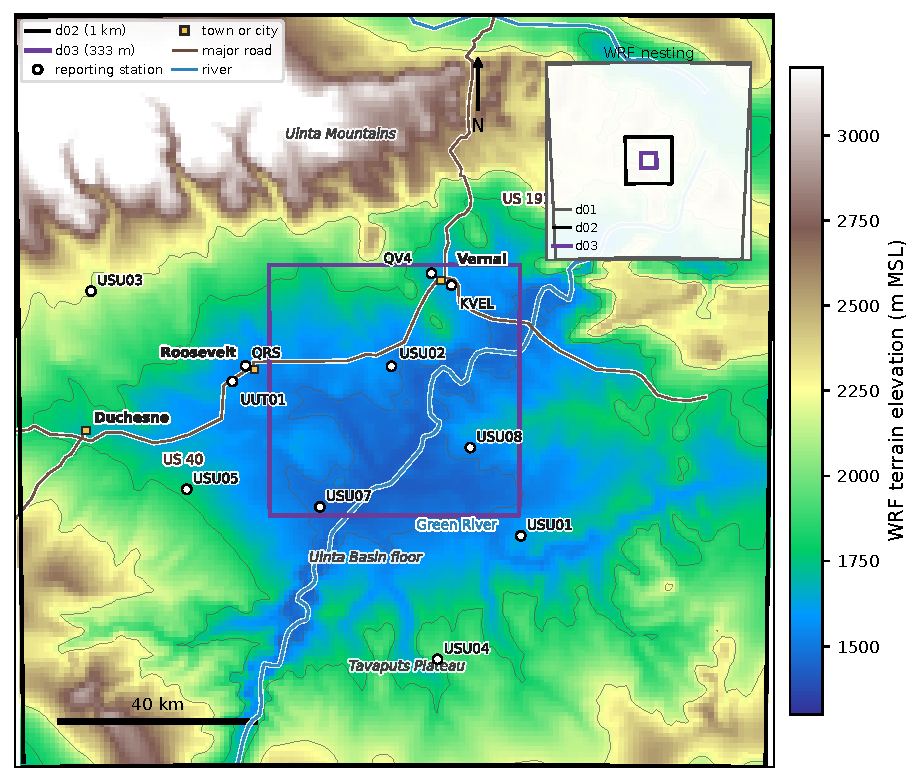
\includegraphics[width=\linewidth]{figures/wrf_geographic_locator_d01_d03.pdf}
\end{minipage}\hfill
\begin{minipage}[t]{0.49\textwidth}
\centering
(\textbf{b})\\[2pt]
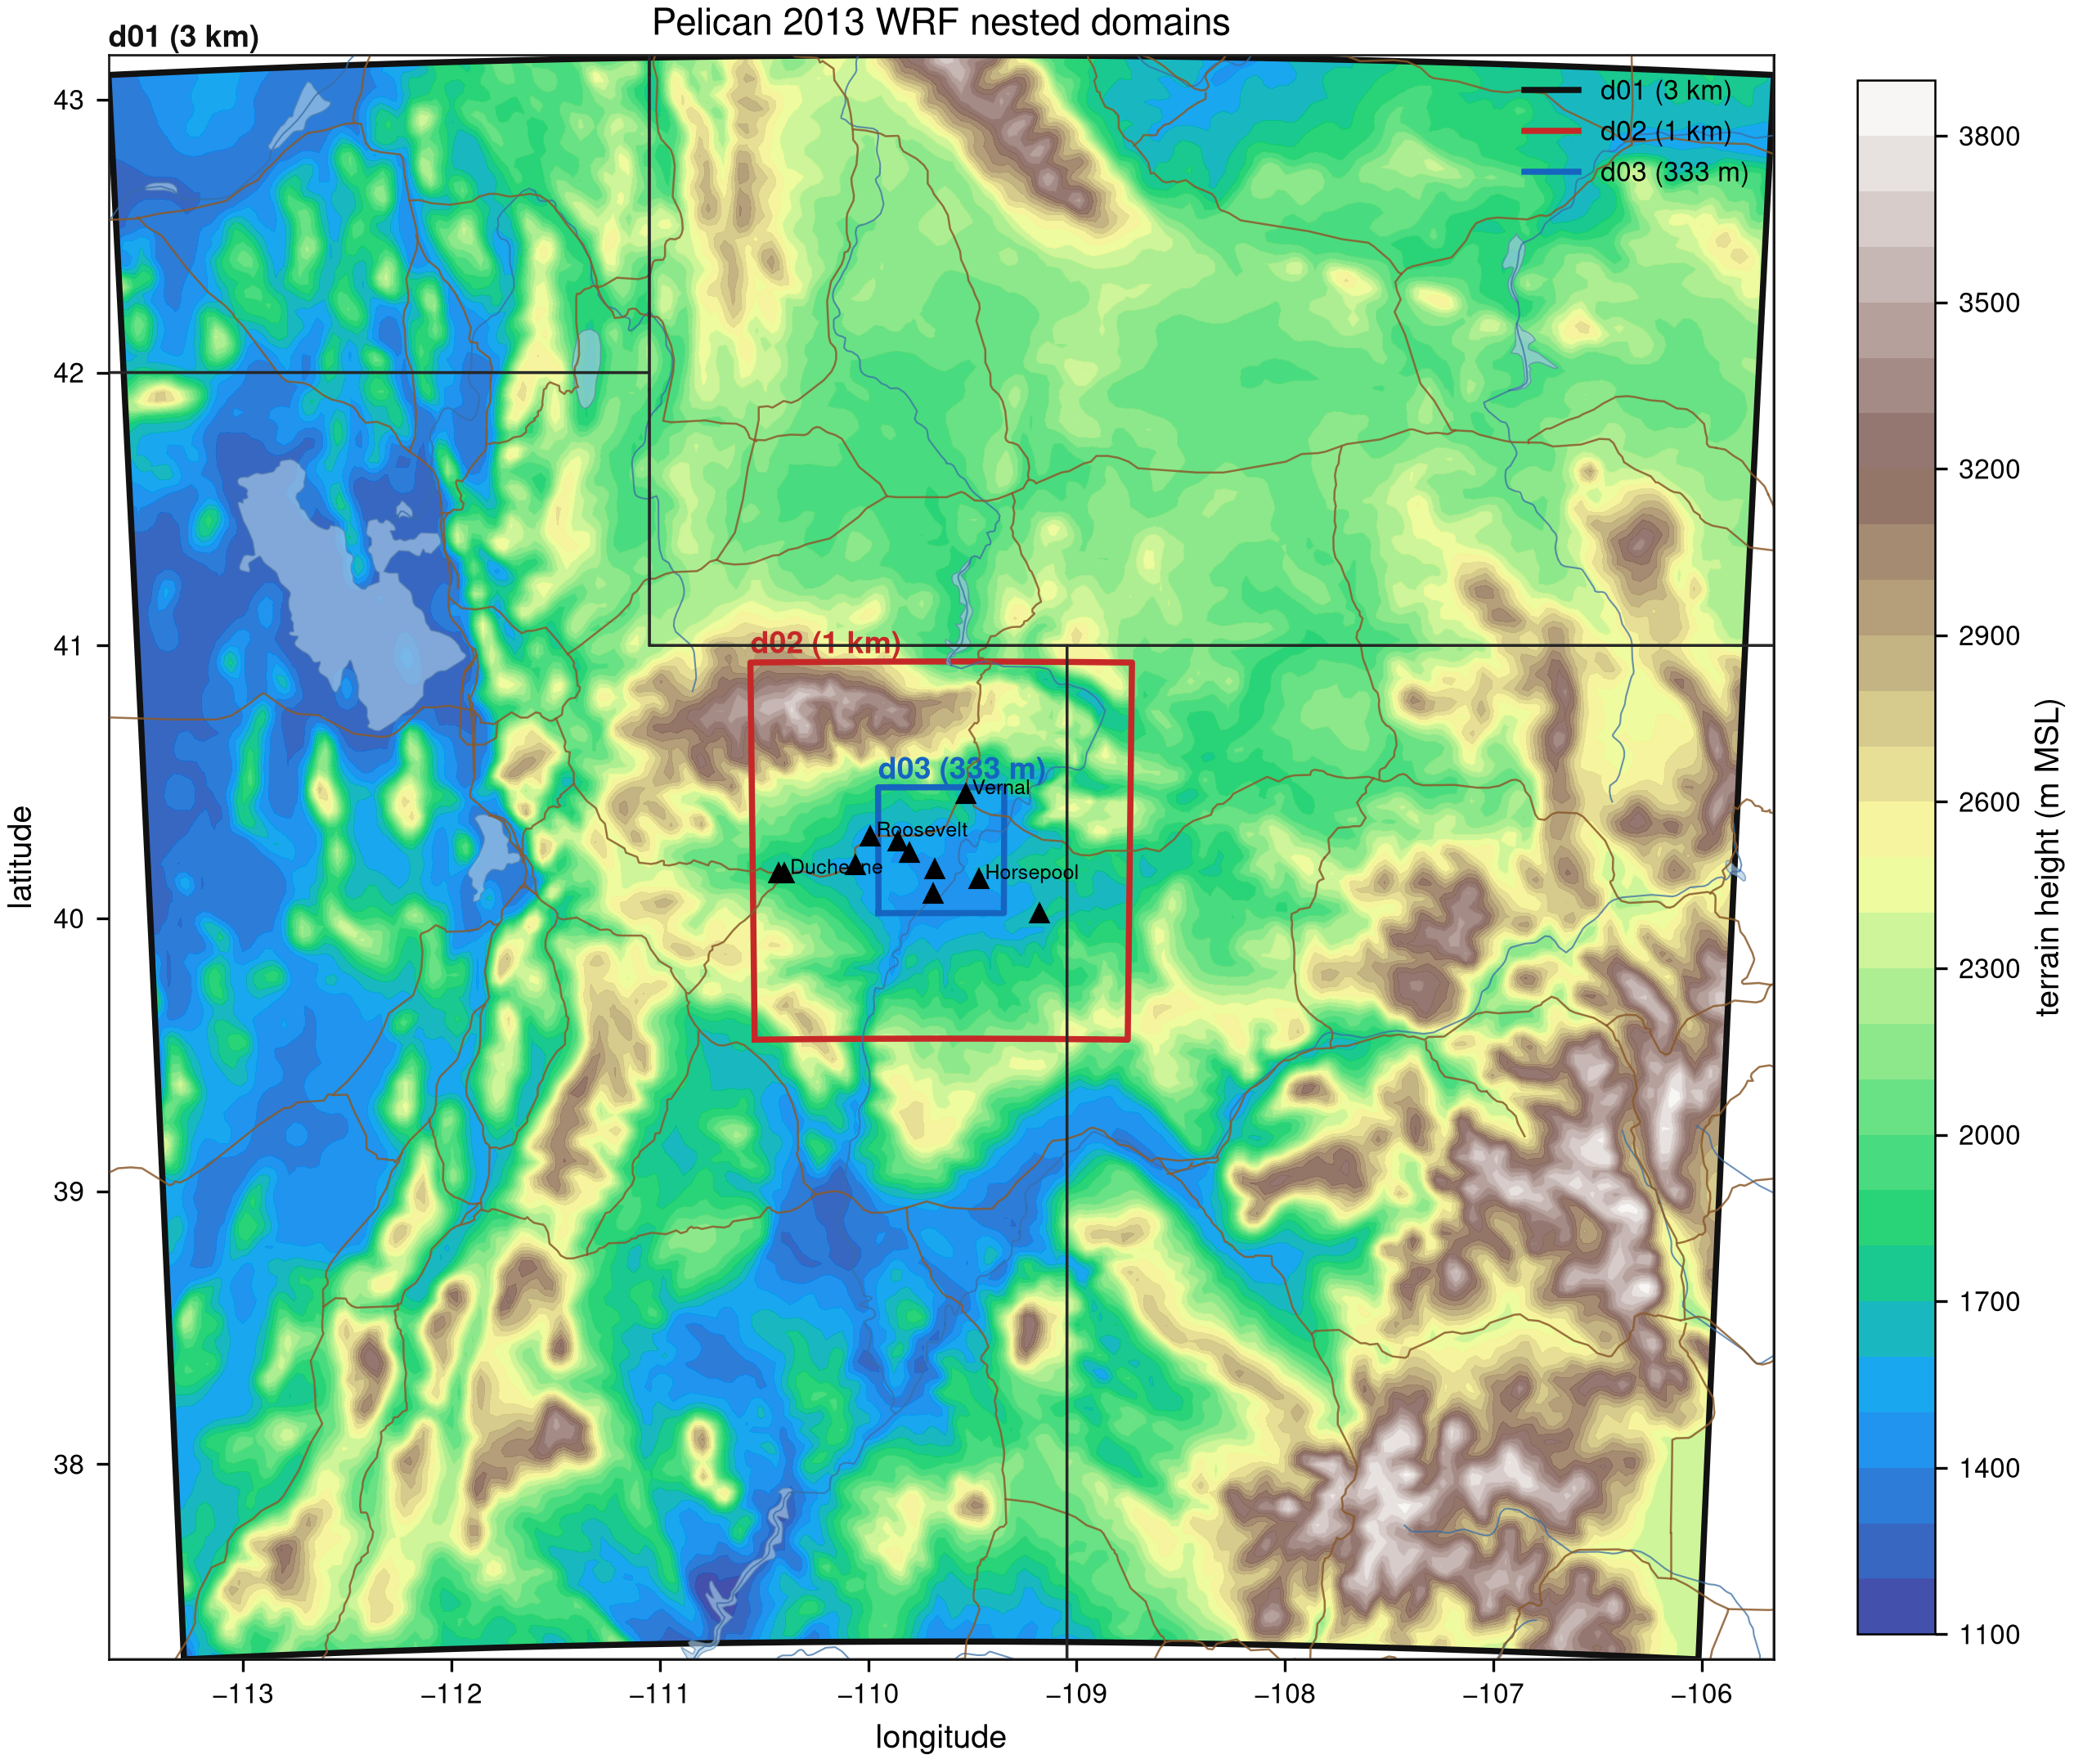
\includegraphics[width=\linewidth]{figures/wrf_nested_domains_d01_d03.png}
\end{minipage}
\caption{\hl{Geographic} %MDPI: Please confirm whether the overlapping content in this figure affects scientific understanding and if it does, please revise it.
% JRL: Confirmed; no overlap affecting scientific understanding.
 and sampling orientation for the evaluation.
(\textbf{a}) The d02 terrain, reporting stations, and~d03 interior define the common evaluation setting.
(\textbf{b}) The d01--d02--d03 WRF grid layout places that setting within the full three-domain configuration.
The d02 domain contains all eleven reporting stations; d03 contains four usable station columns.}
\label{fig:v3-locator}
\end{figure}


\vspace{-12pt}
\begin{figure}[H]

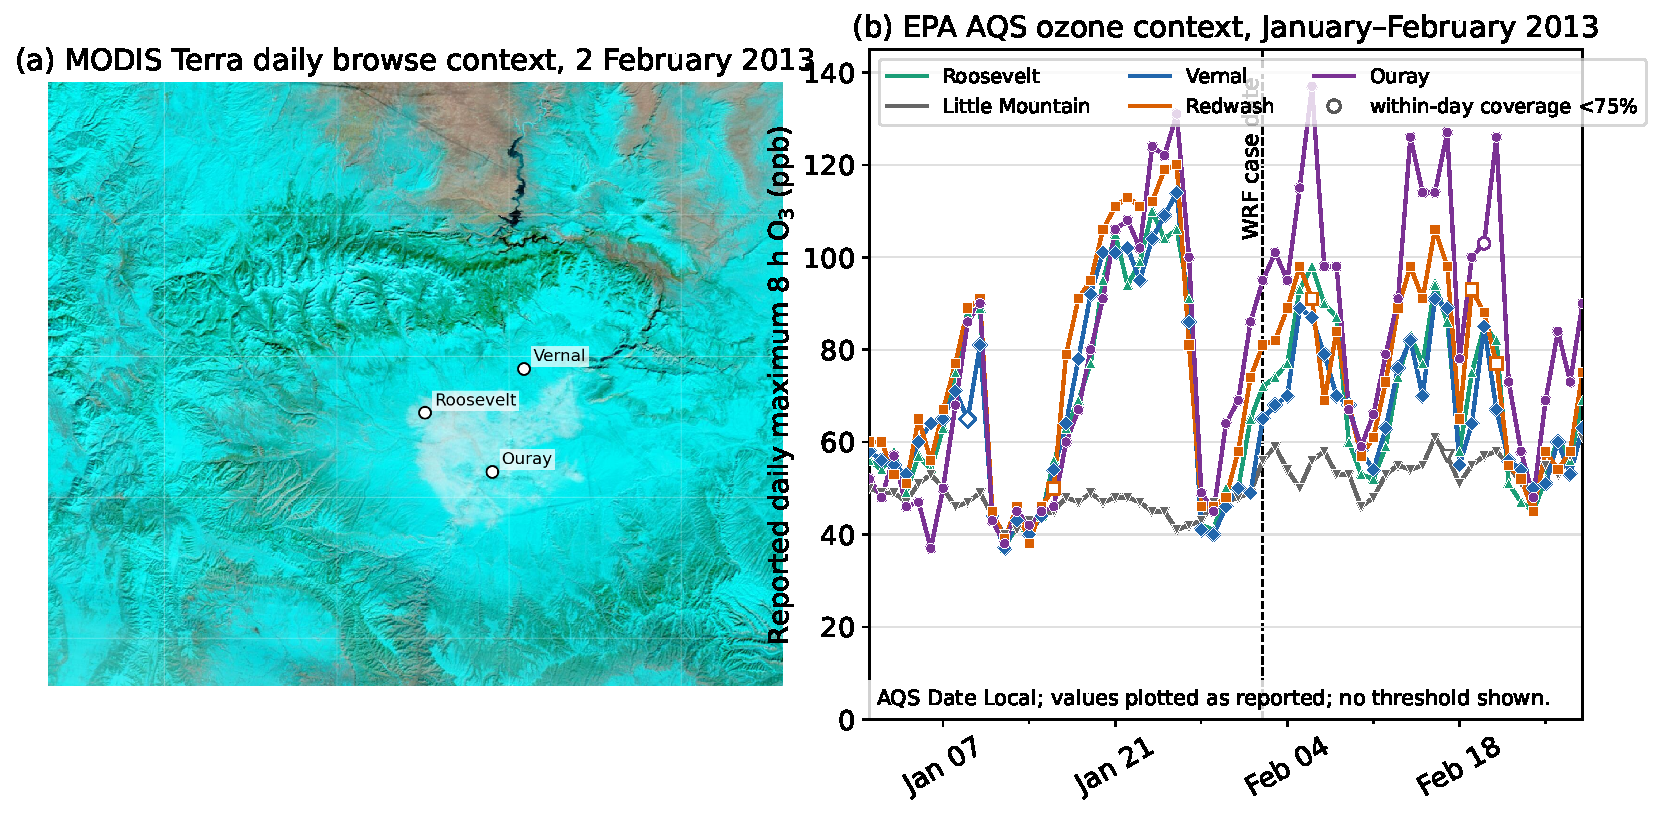
\includegraphics[width=0.93\textwidth]{figures/episode_context_snow_ozone_janfeb2013.pdf}
\caption{\hl{Observed} %MDPI: 1. Please confirm whether the overlapping content in this figure affects scientific understanding and if it does, please revise it.  2. Please confirm whether an explanation of the triangles and squares needs to be added to the figure caption. 3. Figure 2 is not after first citation due to the citation order wrong, please revise citation order and put it after first citation. Same as other figrues, please check all.
% JRL: Marker shapes and placement corrected; size and overlap checked.
 context for the 2 February 2013 simulation date.
(\textbf{a}) NASA GIBS Terra MODIS corrected reflectance, bands 7-2-1, for~the 2 February calendar day; snow and ice generally appear cyan, most liquid cloud appears white, and~ice cloud may also appear cyan.
(\textbf{b}) EPA AQS first maximum value (the eight-hour ozone daily-summary row) at Ouray, Redwash, Roosevelt, Vernal, and~Little Mountain.
Circles, squares, upward triangles, diamonds, and downward triangles identify Ouray, Redwash, Roosevelt, Vernal, and Little Mountain, respectively.
Hollow markers identify the seven site-days with less than 75\% within-day observation coverage.}
\label{fig:v3-episode-context}
\end{figure}


\subsection{WRF Configuration and Archived Simulation~Family}
\label{sec:v3-family}

We used WRF version 4.8.0 \citep{Skamarock2019}, initialised at 1200 UTC with lateral-boundary conditions through 1800 UTC on 2 February 2013.
The inputs were the 1200 and 1800 UTC zero-hour GFS grid 004 (0.5$^{\circ}$; \texttt{gfsanl\_4}) or NAM grid 218 (12~km; \texttt{namanl\_218}) analyses~\citep{GFSAnalysis,NAMAnalysis}.
These integrations include temporally interpolated lateral-boundary forcing, so the retained response combines initial-state and boundary influences.
Three nested domains, d01--d03, have horizontal spacings of 3~km, 1~km, and 333.3~m, with~75 model (eta) levels.
Note that GFS and NAM inputs supply 27 and 40 metgrid levels, respectively.
The WRF grid has approximately 20~m vertical spacing near the surface and a prescribed 50 hPa model top.
The control physics-parametrisation suite comprises Thompson microphysics~\citep{Thompson2008-ti}, Rapid Radiative Transfer Model for General Circulation Models (RRTMG) longwave and shortwave radiation \citep{Iacono2008}, the~revised fifth-generation Pennsylvania State University--National Center for Atmospheric Research Mesoscale Model (MM5) similarity surface layer \citep{Jimenez2012Surface}, the~Noah land-surface model \citep{Tewari2004}, and the Yonsei University (YSU) planetary boundary layer (PBL) scheme \citep{Hong2006}.
No nudging or data assimilation was used.

The terrain datasets were ingested using the WRF Preprocessing System (WPS), version 4.6.0 \citep{Powers2017WRF}.
The default and coarse terrain sources were the 30-arc-second and 5-arc-minute WPS products, respectively, derived from Global Multi-resolution Terrain Elevation Data 2010 (GMTED2010) \citep{DanielsonGesch2011} and distributed by NCAR \citep{WPSGeographicData}.
The fine terrain was a custom 3-arc-second dataset resampled from U.S. Geological Survey (USGS) National Elevation Dataset (NED)/3D Elevation Program (3DEP) 1-arc-second digital elevation models \citep{USGS3DEP1as}.
The fine, default and coarse source spacings correspond to approximately 90~m, 900~m and 9~km north--south spacing at $40^{\circ}$N, distinct from WRF horizontal-grid~spacing.

Table~\ref{tab:v3-family} lists the simulations analysed~here.

\begin{table}[H]
\caption{\hl{Simulations} %MDPI: Please note that changes to the position/size of figures or tables may occur during the production stage, in order to ensure the correct order or readability.
% JRL: Noted; please retain legibility and the order of first citation.
 analysed in this study.
Every run uses WRF 4.8.0, three nests at 3/1/0.333~km with 75 levels, Thompson microphysics, RRTMG radiation, and~Noah land surface unless stated. % JRL: Model version stated here.
``Fine terrain'' is the custom 3-arc-second source, ``default terrain'' is the 30-arc-second class, and~``coarse terrain'' is the 5-arc-minute GMTED2010 source.}
\label{tab:v3-family}

\small
\begin{tabularx}{\textwidth}{LLl}
\toprule
\textbf{Code} & \textbf{Product, Feedback} & \textbf{Terrain and~Physics} \\
\midrule
X0  & NAM, one-way & fine terrain, YSU/MM5 \\
X1  & NAM, one-way & X0 plus slope radiation and~shading \\
X2  & NAM, one-way & X1 with MYJ/Eta instead of YSU/MM5 \\
X3  & NAM, one-way & default-terrain reference~configuration \\
X4  & NAM, one-way & deliberately coarse 5-arc-minute~terrain \\
X5  & NAM, two-way & default~terrain \\
X6  & GFS, two-way & default~terrain \\
X9  & NAM, two-way & X0 with two-way~feedback \\
X10 & GFS, one-way & default~terrain \\
\bottomrule
\end{tabularx}
\end{table}



Hence, our primary comparison crosses GFS and NAM forcing with one-way and two-way feedback on default terrain (X3, X5, X6, and X10).
A controlled contrast pairs runs differing in one configuration choice on the same domain, locations, hours, and diagnostic calculation.
Snow and other land-surface initial fields remain bundled with the forcing product; the Noah scheme is held~fixed.

\subsection{Surface and Common-AGL~Diagnostics}
\label{sec:v3-common-agl}

Surface variables and vertical fields were sampled from the same nearest d02\linebreak   ($\Delta x = 1~\text{km}$ horizontal spacing) column at each station, keeping the model terrain and profile consistent.
The station-to-cell distances are 133--594~m, with~default-terrain elevation offsets of $-32.4$ to $+14.3$~m (\hl{Appendix} %MDPI: We revised the appendix table citation format, please confirm. same as below.
% JRL: Confirmed; please retain this appendix-table citation format throughout.
 \ref{app:v3-data} Table~\ref{tab:v3-stations}).
These pairings retain differences in exposure, slope, and land cover; alternative interpolation methods were not tested.
% Mass-level height above ground level (AGL) was calculated from perturbation plus base geopotential relative to local terrain.
% Winds were destaggered and rotated to earth-relative components.
The potential temperature was interpolated at the layer bounds; wind components were linearly interpolated every 25~m from 50 to 500~m above ground level (AGL) for height integration.
We repeat the eleven-column, five-hour comparison for all nine combinations of 50--500, 50--250, and 100--500~m layers with 10, 25, and 50~m wind integration increments.
The bounds define a common shallow layer rather than an observed inversion~boundary.

The finite-layer potential-temperature difference is defined \hl{as} %MDPI: Reminder: Variables/values; greek letters: please keep them in consistent (italic or normal, bold or not, subscript, superscript) in whole text (including in equations) if necessary. Same for the next occurrences. Please check all equations below.
% JRL: Checked throughout; descriptive pressure subscripts and differential symbols are upright, with variable styling and averaging notation retained.
\begin{equation}
S_{50:500}=\theta(500~\mathrm{m})-\theta(50~\mathrm{m}).
\end{equation}

An increase in potential temperature with height indicates dry static stability \citep{WallaceHobbs2006,Stull1988}.
This bulk difference is a crude tool to locate an inversion top or resolve internal structure: a strong shallow inversion can easily share its profile with an inconspicuous evening.
In addition, the~magnitude of the layer-mean horizontal wind vector was defined as
\begin{equation}
U_{50:500}=\left(\bar{u}^{2}+\bar{v}^{2}\right)^{1/2},
\end{equation}
where the bars denote the height means from 50~m to 500~m AGL, not temporal or turbulent averages.
We also calculate the layer-mean scalar speed $\overline{(u^{2}+v^{2})^{1/2}}$ and the vector-to-scalar ratio to assess cancellation between winds at different heights.

\subsection{Pairing, Aggregation, and~Short-Sample~Sensitivity}
\label{sec:v3-aggregation}

The coding language Python was used for analysis and acquisition of data. Specifically, Herbie 2026.3.0 \citep{Herbie} and SynopticPy 2026.6.0 \citep{SynopticPy} were used for source-data retrieval and Synoptic API access, respectively.
Analysis and plotting were performed using \hl{NumPy} 2.5.0 %MDPI: Please state which version of the software was used. Same as below.
% JRL: Retrieval, analysis, plotting versions now stated from the environment records.
 \citep{Harris2020NumPy}, \hl{SciPy} 1.18.0 \citep{Virtanen2020SciPy}, \hl{pandas} 3.0.3~\citep{McKinney2010}, Polars 1.42.0 \citep{Polars}, \hl{xarray} 2026.4.0 \citep{HoyerHamman2017}, and \hl{Matplotlib} 3.11.0 \citep{Hunter2007Matplotlib}.
The later label revisions to the controlled-comparison and station-column figures used Matplotlib 3.10.8.

Run differences were paired by location and valid hour, and then reduced to one spatial median per hour.
The reported five-hour effects are means of those medians.
To explore temporal sensitivity \citep{Wilks2019}, a~circular moving-block calculation drew 20,000 resamples of the five medians using two-hour blocks.
Its 2.5th and 97.5th percentiles are descriptive sensitivity bounds for this single case; we emphasise the practical effect size without treating them as evidence of statistical~significance.

\subsection{Area-Integrated Heat~Deficit}
\label{sec:v3-heatdeficit-methods}

To represent the cold-pool strength numerically, we adapted the basin heat-deficit formulation of Whiteman et al. \citep{Whiteman1999} and the column implementation of Adler et al. \citep{Adler2023}.
Using the hydrostatic balance, $\mathrm{d}p=-\rho g\,\mathrm{d}z$, to~express the column mass in pressure coordinates~\citep{WallaceHobbs2006}, we defined
\begin{equation}
H=\frac{c_{p}}{g}\int_{p_{\mathrm{c}}}^{p_{\mathrm{s}}}\max\{\theta_{\mathrm{crest}}-\theta(p),0\}\,\mathrm{d}p,
\end{equation}
where $c_{p}$ is the dry-air specific heat at constant pressure, $g$ is the gravitational acceleration, and~$p_{\mathrm{s}}>p_{\mathrm{c}}$ are the surface and crest-reference pressures.
The reference potential temperature is interpolated to the fixed crest height in each modelled column; clipping retains only positive deficits.
This potential-temperature proxy then describes stratification relative to that reference.
We report its cell-area-weighted mean in MJ~m$^{-2}$: the primary area is the convex hull of eleven stations and eleven basin waypoints, restricted to terrain below 2200~m (4965 d02 cells covering 5277~km$^{2}$).
We tested the sensitivity of the results to this hull at 2100, 2200, and 2300~m; increasing or eroding the area by one cell; and in station-only areas at 2200~m.
Given the sensitivity of the case to complex terrain, we ensure that the GFS--NAM contrasts share a terrain~dataset.

\section{Results}
\label{sec:v3-results}


\subsection{Observed Episode~Context}
\label{sec:v3-episode-context}

The MODIS image shows extensive snow and ice across the basin and surrounding terrain (Figure~\ref{fig:v3-episode-context}a).
The AQS series places 2 February within a broader period of elevated ozone, with~daily maximum eight-hour concentrations of 56--95~ppb across the five sites (Figure~\ref{fig:v3-episode-context}b).
These observations establish episode context without attributing ozone to the simulated~meteorology.


\subsection{Observed Surface-Temperature~Context}
\label{sec:v3-observed-context}

Inspecting a sample of observation stations across a range of altitudes, we found that a~representative basin-floor station repeatedly separated from the higher sites between 31 January and 3 February, with~a strong variation in diurnal temperature differences (Figure~\ref{fig:v3-observed}).
Seep Ridge (USU04; 1933~m) appears anomalous, despite a modest station-to-cell distance of 133~m and 3~m terrain offset in the vertical, showing latent limitations in estimating cold-pool strength with observations.
Exposure, slope flow, and representativeness are possible explanations, but~the metadata do not distinguish them.
Indeed, all samples were obtained without failing a pre-processing quality-control check.
The recurring floor-to-bench separation is consistent with a cold-pool surface pattern; however, the~horizontally separated sites cannot determine its vertical~structure.
\vspace{-3pt}
\begin{figure}[H]

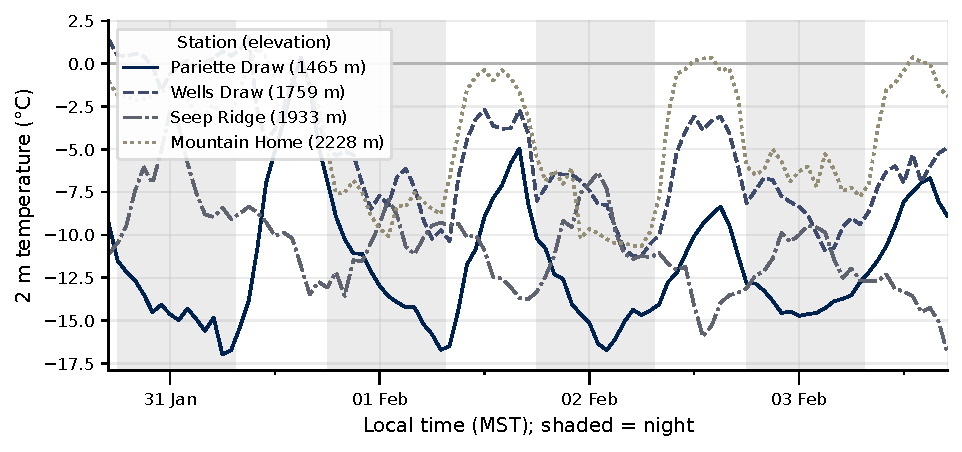
\includegraphics[width=0.9\textwidth]{figures/obs_temp_timeseries_feb0102.pdf}
\caption{\hl{Observed} %MDPI: Please confirm whether the overlapping content in this figure affects scientific understanding and if it does, please revise it.
% JRL: Confirmed; no overlap affecting scientific understanding.
 2 m temperature evolution at four elevation-spanning Uinta Basin stations from 31 January through 3 February 2013.
Shading indicates approximate local night.
The series show a spatial surface-temperature pattern, not a co-located vertical profile.}
\label{fig:v3-observed}
\end{figure}


\subsection{Overview of Experiment~Responses}
\label{sec:v3-effects-panel}

The forcing-product contrasts give the largest temperature and layer-mean wind responses (Figure~\ref{fig:v3-effects}).
The PBL/surface-layer response is smaller; slope-radiation and feedback interaction effects cluster near zero on these scales.
Pressure and wind-error metrics have inconsistent trends in time, preventing an overall configuration ranking for this~case.



\subsection{Driving-Product Response in the Lower~Layer}
\label{sec:v3-driving-response}

Runs forced with GFS produced a smaller 50--500~m potential-temperature difference than NAM under both feedback modes (Figure~\ref{fig:v3-retention}).
Paired GFS-minus-NAM effects averaged $-3.63$~K with two-way feedback and $-3.65$~K with one-way feedback, consistently borne out by a constant sign at every hour (Table~\ref{tab:v3-effects}).
The layer-mean wind-vector magnitude increased by 0.79 and 0.99~m~s$^{-1}$, respectively, also with consistent hourly signs.
Scalar-speed differences were similar, and~directional cancellation therefore likely does not create the speed ordering (\hl{Appendix} \ref{app:v3-data} Table~\ref{tab:v3-wind-cancellation}).
The vector-to-scalar ratio difference was not consistent and hence not analysed~further.

% JRL: Figure 4 moved after the first paragraph of Section 3.4 to use the preceding page space.
\vspace{-6pt}
\begin{figure}[H]

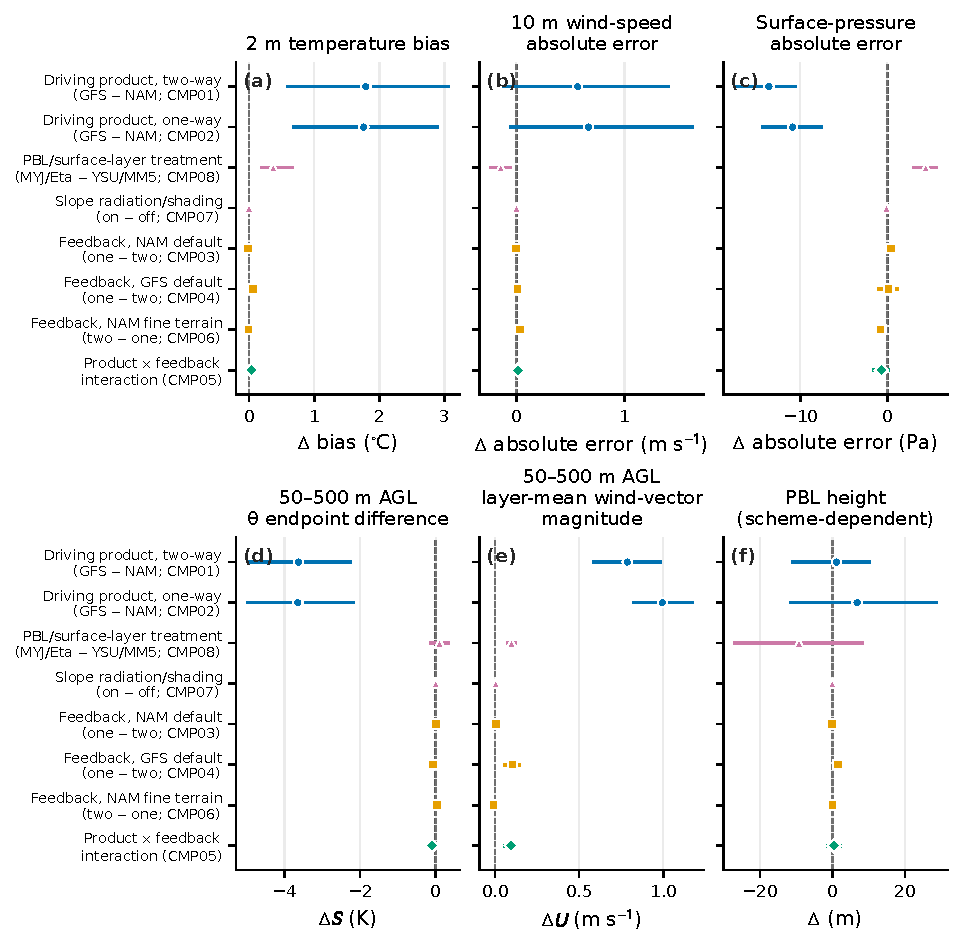
\includegraphics[width=0.98\textwidth]{figures/fig_common_pipeline_effects.pdf}
\caption{\hl{Mean} %MDPI: Please note that each subfigure should be described separately in the caption., e.g., (a) xxx; (b) xxx.
% JRL: All six panels are now described separately; the descriptive whisker explanation is retained.
 five-hour effects for the controlled comparisons that share the station/common-AGL pipeline.
(\textbf{a}) 2 m temperature bias ($^{\circ}$C); (\textbf{b}) 10 m wind-speed absolute error (m s$^{-1}$); (\textbf{c}) surface-pressure absolute error (Pa); (\textbf{d}) 50--500 m AGL potential-temperature endpoint difference (K); (\textbf{e}) layer-mean wind-vector magnitude (m s$^{-1}$); and (\textbf{f}) native PBL height (m).
Colours and marker shapes identify forcing-product, feedback, and~interaction contrasts.
Whiskers show descriptive sensitivity intervals for five dependent hourly medians.}
\label{fig:v3-effects}
\end{figure}

The GFS-minus-NAM wind differences retain their respective signs in every hour across all nine layer/increment combinations, indicating a consistent pattern.
Their magnitudes depend on layer bounds (\hl{Appendix} \ref{app:v3-data} Table~\ref{tab:v3-layer-sensitivity}); varying the integration increment at fixed bounds changed the mean paired wind effects by less than 0.02~m~s$^{-1}$.
This tests the integration sampling of the same linearly interpolated winds, rather than the native vertical resolution or an alternative interpolation method.
Native PBL-height differences change sign under both feedback modes, consistent with the diagnostic's scheme dependence discussed by \mbox{Tran et al. \citep{Tran2018FDDA}}.
\vspace{-3pt}
\begin{figure}[H]

% JRL: Figure 5 reduced to better accomodate text.
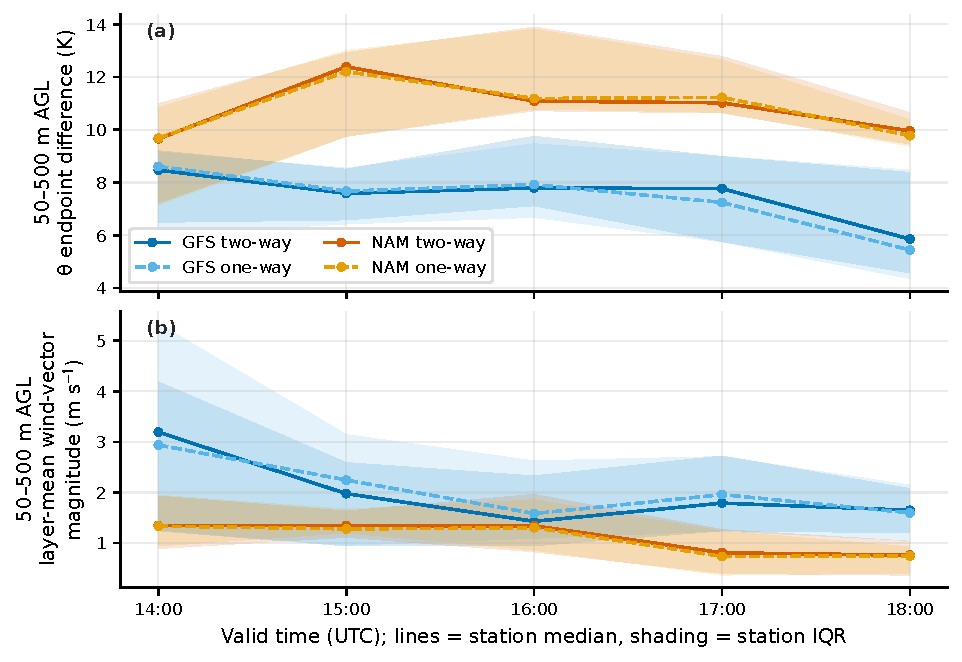
\includegraphics[width=0.65\textwidth]{figures/wrf_retention_ventilation_d02_14to18.pdf}
\caption{\hl{Station-column} %MDPI: 1. Please note that each subfigure should be described separately in the caption., e.g., (a) xxx; (b) xxx.  2. Please confirm whether an explanation of the shadow area needs to be added to the figure caption.
% JRL: Both panels, station medians, and shaded interquartile ranges are now explained.
 medians and interquartile ranges for the 50--500 m AGL potential-temperature endpoint difference and layer-mean wind-vector magnitude over the matched window.
(\textbf{a}) Potential-temperature endpoint difference; (\textbf{b}) layer-mean wind-vector magnitude.
Lines show station medians; shading shows the station interquartile range.
Solid lines denote two-way feedback and dashed lines denote one-way feedback.
Both feedback modes retain the GFS--NAM ordering throughout the window.}
\label{fig:v3-retention}
\end{figure}


\subsection{Surface and Spatial~Corroboration}
\label{sec:v3-surface}

Runs forced with GFS were warmer at the surface than NAM, consistent with the common-layer diagnostics (Table~\ref{tab:v3-surface-summary}).
The 2~m temperature-bias contrasts were approximately +1.8~$^{\circ}$C under both feedback modes.
The pressure's absolute error decreased, while the hourly wind-error differences followed no strong pattern.
Figure~\ref{fig:v3-bulk-theta} compares the observed bench-minus-floor surface index with the two-way-feedback~simulations.
\vspace{-3pt}
\begin{figure}[H]

% JRL: Figure 6 reduced to better fit text.
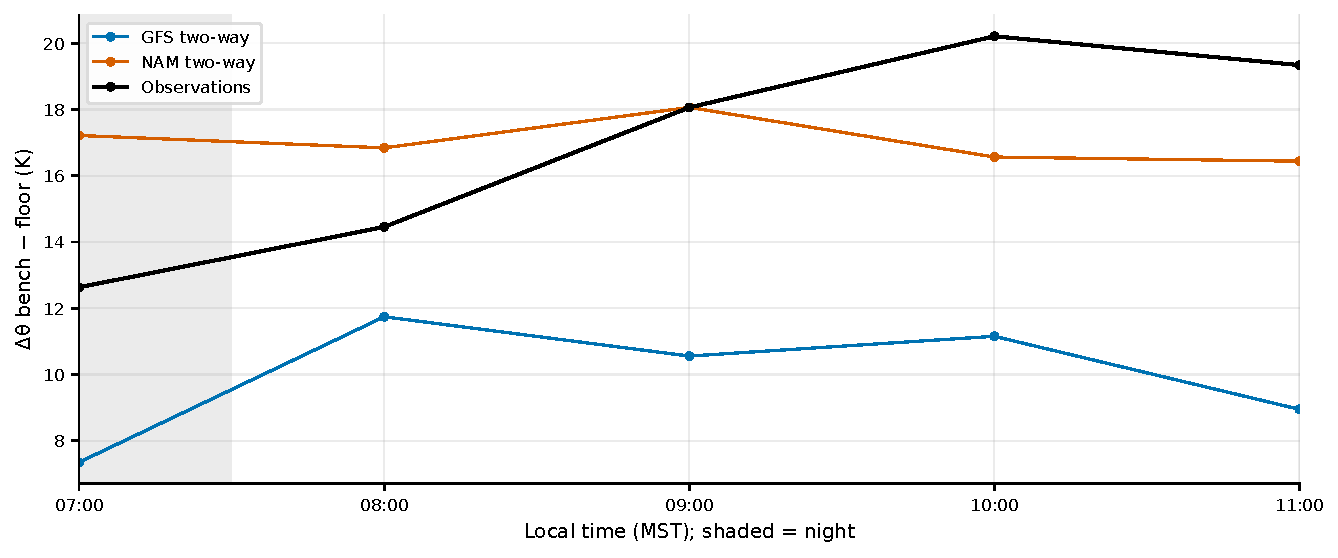
\includegraphics[width=0.65\textwidth]{figures/wrf_inversion_index_feb0102_gfs2way_vs_nam2way_d02_14to18.pdf}
\caption{\hl{Observed} %MDPI: Please confirm whether an explanation of the shadow area needs to be added to the figure caption.
% JRL: Shading indicates approximate local night; this is now stated in the caption.
 and modelled Mountain Home-minus-Pariette Draw surface potential-temperature contrast from 1400 to 1800 UTC on 2 February 2013.
The modelled series are X6 (GFS two-way) and X5 (NAM two-way) on d02, sampled at the same five hours as the observations.
The index is a horizontally separated bench-minus-floor surface contrast.
Shading indicates approximate local night.}
\label{fig:v3-bulk-theta}
\end{figure}

The five-hour mean bench-minus-floor contrast was 16.94~K observed, 17.03~K in X5 (NAM two-way), and~9.95~K in X6 (GFS two-way).
Across the area of interest, GFS-minus-NAM near-surface responses were positive on average and concentrated below 500~m AGL under both feedback modes (Table~\ref{tab:v3-surface-summary}).

\subsection{Heat~Deficit}
\label{sec:v3-heatdeficit}

Runs driven by GFS retained a lower area-mean heat deficit at every hour in all sensitivity tests (i.e., changing the area's footprint), with~mean paired effects of approximately $-1.2$~MJ~m$^{-2}$ under both feedback modes (Table~\ref{tab:v3-heatdeficit}).
Every run ended with a greater deficit at 1800 than at 1400 UTC, despite intermittent within-window declines (Figure~\ref{fig:v3-heatdeficit-traj}).
\vspace{-3pt}
\begin{figure}[H]

% JRL: Figure 7 reduced to accomodate text.
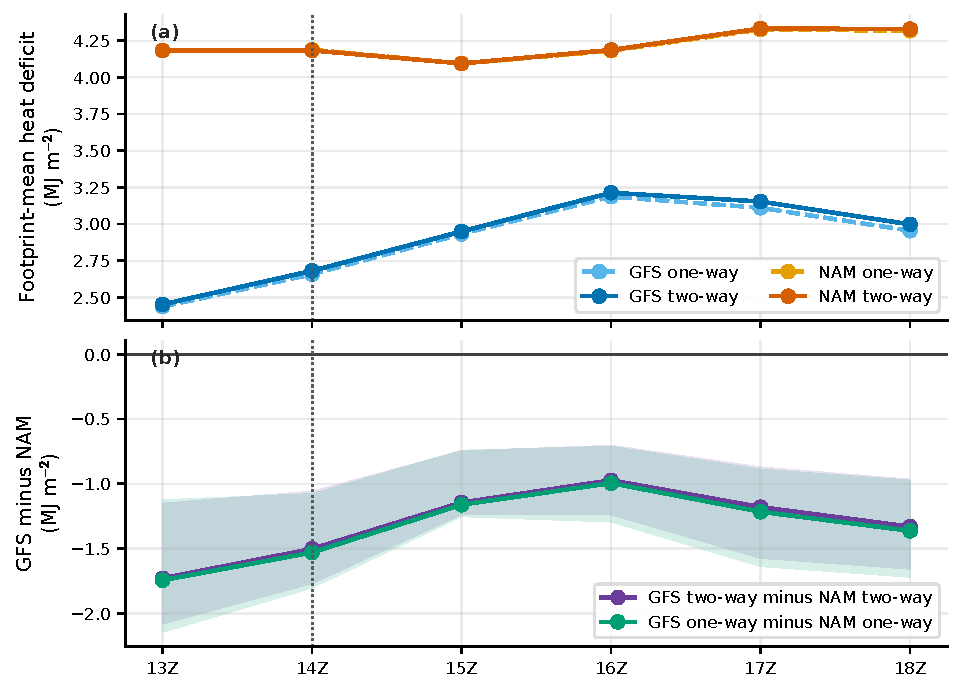
\includegraphics[width=0.72\textwidth]{figures/wrf_heat_deficit_d02_13to18.pdf}
\caption{\hl{Footprint-mean} %MDPI: 1. Please note that each subfigure should be described separately in the caption., e.g., (a) xxx; (b) xxx.  2. Please confirm whether an explanation of the shadow area needs to be added to the figure caption.
% JRL: Both panels and the shaded sensitivity envelope are now explained.
 heat-deficit trajectories for the four default-terrain matrix members and seven-definition sensitivity envelopes for the two GFS-minus-NAM pairs.
(\textbf{a}) Four-run trajectories for the primary 2200 m crest footprint; (\textbf{b}) feedback-matched GFS-minus-NAM contrasts for that footprint, with shading spanning the minimum to maximum across the seven footprint definitions.
The 1300 UTC values orientate the trajectories but are excluded from every reported criterion and effect.
GFS-driven runs retain a smaller deficit throughout, but~the deficit does not decline faster in either GFS-based member.}
\label{fig:v3-heatdeficit-traj}
\end{figure}


\subsection{Fine-Terrain~Experiments}
\label{sec:v3-process}

Replacing YSU/revised-MM5 with Mellor--Yamada--Janji\'c (MYJ)/Eta schemes \citep{Janjic1994} on fine terrain with slope radiation (X2 minus X1) increased the temperature bias by 0.37~$^{\circ}$C, reduced the wind absolute error by 0.145~m~s$^{-1}$, and increased the layer-mean wind-vector magnitude by 0.098~m~s$^{-1}$.
All changes were consistent in the 5 h period, but~were smaller than the forcing-product impact.
The inconsistent temperature- and wind-error changes preclude further commentary on the overall scheme~behaviour.

Adding slope radiation and shading (X1 minus X0) had negligible effects at basin-floor station columns but produced a spatially organised sidewall skin-temperature~response.

\subsection{Nest-Feedback and Terrain~Fineness}
\label{sec:v3-feedback}

\label{sec:v3-cmp06}
Effects introduced by toggling domain two-way feedback were small for both products: the one-way minus two-way contrasts were at most 0.07~K in bulk potential-temperature difference and 0.10~m~s$^{-1}$ in wind-vector magnitude (Table~\ref{tab:v3-effects}).
The fine-terrain NAM comparison (X9 minus X0, two-way minus one-way) was similarly small, with~sensitivity bounds spanning zero for both metrics.
The surface wind and pressure changes were negligible, providing no feedback recommendation beyond this~case.

\subsection{Terrain-Source~Tests}
\label{sec:v3-terrain}

The terrain comparisons hold NAM forcing, one-way feedback, WRF grid spacing, and YSU/MM5 physics fixed as control.
A default-minus-fine (X3 minus X0) experiment had a small d02 response, while a wider default-minus-coarse (X3 minus X4) and fine-minus-coarse (X0 minus X4) terrain experiment gave larger spatial responses.
For fine minus coarse at 1600 UTC, the~heat-deficit median changed sign between d02 (+0.014~MJ~m$^{-2}$) and d03 ($-0.184$~MJ~m$^{-2}$), while the two d03 section medians were +0.278 and +0.369~K.
Figure~\ref{fig:v3-terrain-cmp11} shows this domain-dependent response without obviously benefitting from finer~terrain.
\vspace{-3pt}
\begin{figure}[H]

% JRL: Figure 8 reduced for better spacing.
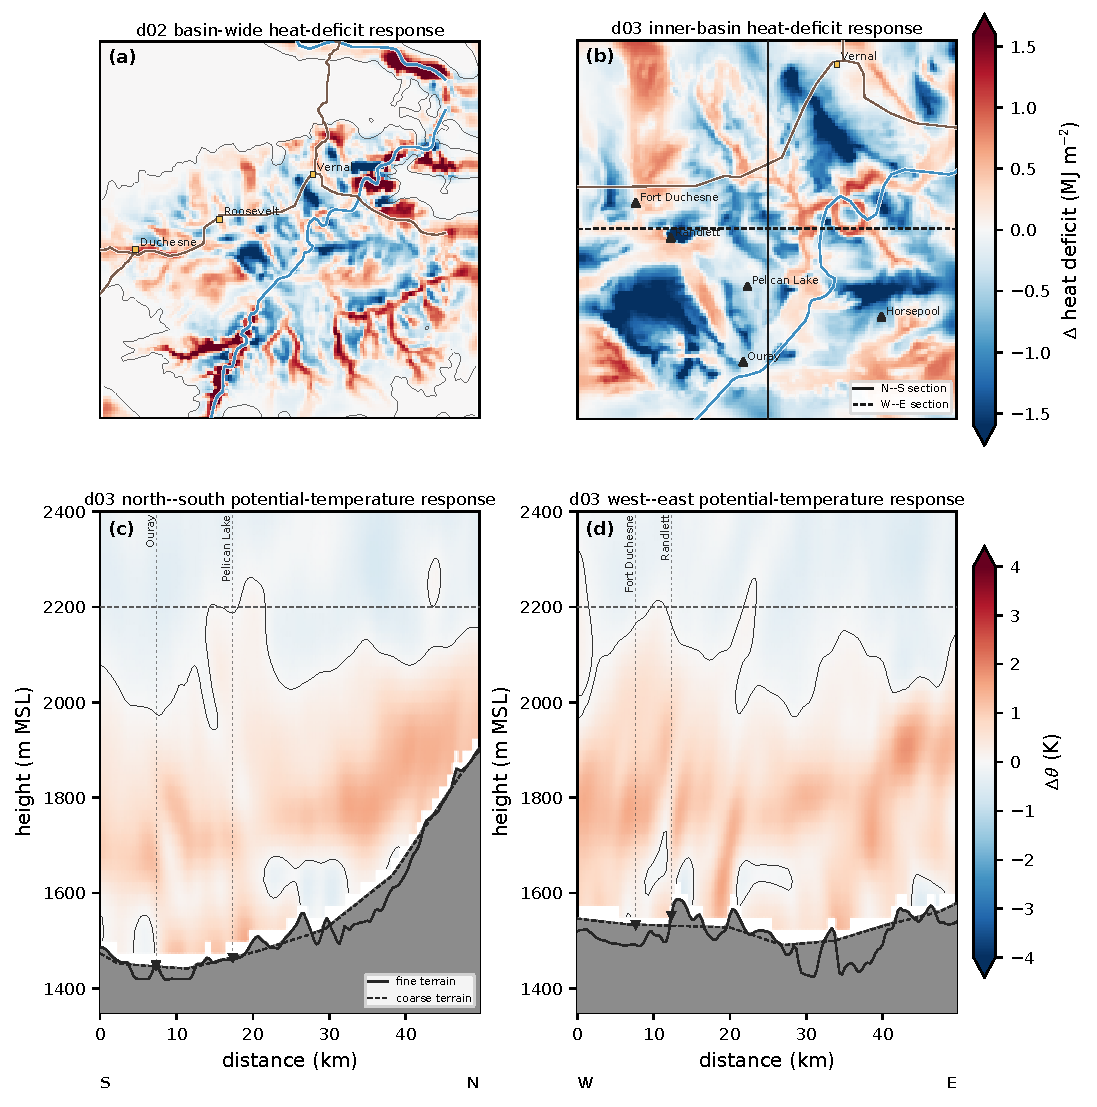
\includegraphics[width=0.90\textwidth]{figures/wrf_terrain_cmp11_d02_d03_16z.pdf}
\caption{\hl{Diagnostic} %MDPI: 1. Please confirm whether the overlapping content in this figure affects scientific understanding and if it does, please revise it.  2.  Please confirm whether an explanation of the dashed line needs to be added to the figure caption.
% JRL: Dashed lines explained; overlap checked on the previous proof, and size now reduced.
 response to the widest controlled terrain comparison at 1600 UTC, calculated as X0 minus X4 (fine 3-arc-second minus coarse 5-arc-minute source).
(\textbf{a}) The basin-wide d02 and\linebreak   (\textbf{b}) inner-basin d03 top-down heat-deficit maps share a fixed $\pm1.6$ MJ m$^{-2}$ scale.
(\textbf{c}) The north--south and (\textbf{d}) west--east d03 lower-atmosphere potential-temperature sections share a fixed $\pm4$ K scale and the 2200 m crest reference.
In (\textbf{b}), solid and dashed lines locate the north--south and west--east sections, respectively.
In (\textbf{c},\textbf{d}), dashed terrain lines show coarse terrain, the horizontal dashed line marks the 2200 m crest reference, and vertical dashed lines mark labelled waypoints.}
\label{fig:v3-terrain-cmp11}
\end{figure}


\section{Discussion}
\label{sec:v3-discussion}


\subsection{Forcing-Product Differences in the Lower~Layer}
\label{sec:v3-disc-supplied-state}

The principal result is the GFS--NAM separation under both feedback settings: the GFS has a smaller vertical potential-temperature bulk differences, larger layer-mean wind-vector magnitude, and~lower heat deficit (weaker modelled cold pool).
These differences matter for the meteorology supplied to a chemistry model, but~do not measure the precursor confinement or residence time.
Because emissions, snow, cloud, and~photolysis/chemical-mechanism errors can compensate in coupled simulations \citep{Ahmadov2015Complete,Neemann2015-ws,Matichuk2017-bq}, forcing-product sensitivity deserves focus in future air-chemistry simulations; ensemble experiments across multiple cases would test its~generality.

The modelled d03 Horsepool profiles, sampled near the lowest point in the Basin (and cold-air sink), show product-specific initial states and first-hour evolution (Figure~\ref{fig:v3-spinup-profiles}).
The early profile differences reinforce the need to assess the meteorological inputs before adding chemistry, but~cannot separate initial-state influence from lateral-boundary~evolution.
 \vspace{-3pt}
\begin{figure}[H]
% JRL: Figure 9 panels slightly reduced.

\begin{minipage}[t]{0.45\textwidth}
\centering
(\textbf{a})\\[2pt]
\IfFileExists{figures/theta_profiles_horsepool_gfs_nam_12z.pdf}{%
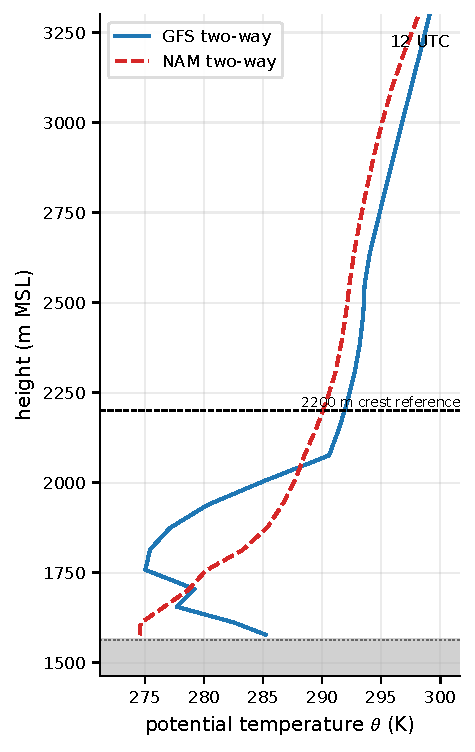
\includegraphics[width=\linewidth]{figures/theta_profiles_horsepool_gfs_nam_12z.pdf}%
}{\fbox{\parbox[c][0.28\textheight][c]{0.88\linewidth}{\centering X6 and X5 Horsepool profiles at 1200 UTC.}}}
\end{minipage}\hfill
\begin{minipage}[t]{0.45\textwidth}
\centering
(\textbf{b})\\[2pt]
\IfFileExists{figures/theta_profiles_horsepool_gfs_nam_13z.pdf}{%
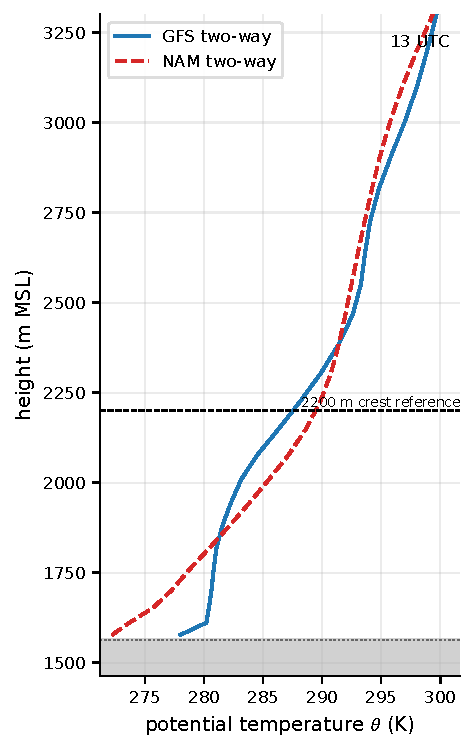
\includegraphics[width=\linewidth]{figures/theta_profiles_horsepool_gfs_nam_13z.pdf}%
}{\fbox{\parbox[c][0.28\textheight][c]{0.88\linewidth}{\centering X6 and X5 Horsepool profiles at 1300 UTC.}}}
\end{minipage}
\caption{Model d03 ($\Delta x = 333.3~\text{m}$) potential-temperature profiles at Horsepool for X6 (GFS) and X5 (NAM).
(\textbf{a}) The 1200 UTC initialised states and (\textbf{b}) the 1300 UTC one-hour forecasts use identical axes.
Grey shading marks levels below the local model terrain, and~the dashed 2200 m line is the fixed crest reference rather than an observed cold-pool top.}
\label{fig:v3-spinup-profiles}
\end{figure}


\subsection{Heat-Deficit Evolution and Spatial~Extent}
\label{sec:v3-disc-spatial}

A lower GFS-run heat deficit persisted across all footprint sensitivity tests, but~positive net changes in every run do not demonstrate faster cold-pool erosion during the retained window.
Indeed, at~least a full diurnal cycle is needed to test differences in cold-pool erosion or persistence, and~is a topic of the authors' current research.
The forcing-product response was strongest below 500~m AGL and consistent in its mean effect, while its early spatial sign share fell below the predeclared two-thirds criterion (Table~\ref{tab:v3-surface-summary}).

\subsection{Parametrisation, Feedback, and~Terrain~Sensitivities}
\label{sec:v3-disc-process}

Parametrisation and feedback effects were smaller than the forcing-product response effect on the temperature and wind diagnostics.
The changes in parametrisation configuration modulated wind error while increasing temperature separation; feedback remained small on both terrain branches.
While the changes were small, slope radiation and terrain-fineness effects produced spatial responses that in situ stations could miss.
These results favour combining station and spatial diagnostics for a fully three-dimensional analysis (and advancing in time).
Finer terrain can reveal geometric detail hidden by a coarse representation, as~illustrated by scale-dependent measurements of irregular boundaries \citep{Mandelbrot1967-gq}.
That analogy does not establish aerodynamic roughness or drainage speed in WRF; whether finer terrain changes cold-air pathways or storage remains a question for targeted~experiments.

\subsection{Observational and Design~Limits}
\label{sec:v3-disc-domains}

A bounded search of accessible holdings found no measured in-basin profile within the exact retained window.
A provisional Roosevelt sounding began at 1801:54 UTC \citep{UtahUBOS}, just after the window, and~has not undergone scientific QC or matched WRF analysis; inaccessible holdings were not treated as empty.
Thus the surface comparisons do not validate inversion depth or free-air vertical structure.
Separating initial from lateral forcing requires new experiments, while nudging tests require independent observations withheld from assimilation.
Longer matched runs and additional cases are needed to assess persistence and~generality.

\section{Conclusions}
\label{sec:v3-conclusions}

We have presented WRF experiments to highlight the sensitivity of cold-pool representation---relevant to the retention of ozone and its precursors---to combined initial and lateral weather-model forcing.
We use a well documented winter 2013 case, notoriously for its poorly simulated meteorology, in the Uinta Basin to identify differences among the meteorological simulations.
The GFS--NAM contrast produced the largest repeated lower-layer response on the d02 (1 km) domain.
Under both feedback modes, GFS-driven runs were warmer at the evaluated surface sites and had an approximately 3.6~K smaller 50--500~m potential-temperature difference, a\linebreak   0.8--1.0~m~s$^{-1}$ larger wind-vector magnitude, and an approximately 1.2~MJ~m$^{-2}$ lower area-mean heat deficit (weaker cold pool).
The heat-deficit differences representsa state offset without demonstrated faster cold-pool~erosion.

Nest-feedback effects were small (at most 0.07~K and 0.10~m~s$^{-1}$ on the same layer metrics), while MYJ/Eta increased the temperature bias by 0.37~$^{\circ}$C and reduced the wind absolute error by 0.145~m~s$^{-1}$.
The slope radiation and terrain effects depended on the spatial definition: the fine-minus-coarse heat-deficit median changed from +0.014~MJ~m$^{-2}$ on d02 to $-0.184$~MJ~m$^{-2}$ on d03.
These findings support complementary station, layer, and basin-wide diagnostics for meteorology supplied to chemistry models, followed by ensemble experiments across multiple cases to examine uncertainty.
Targeted forcing experiments, longer matched integrations, and independent vertical observations are needed to identify forcing contributions and evaluate inversion depth and persistence; this study establishes neither basin export nor ozone response.
Appendix~\ref{app:v3-data} retains numerical summaries and sampling metadata for~reproducibility.

\appendixtitles{yes}
\appendixstart
\appendix
\section{Data Tables and Secondary~Diagnostics}
\label{app:v3-data}

\vspace{-3pt}
\begin{table}[H]
\caption{Case-window temperature stations and nearest d02 sampling audit.
Coordinates (rounded to three decimal places) and reported elevations are from the registered Synoptic Data PBC metadata; separation is great-circle distance to the sampled cell centre, and~the final column is X3 default-terrain model height minus reported station elevation.}
\label{tab:v3-stations}
% JRL: Confirmed; the revised Table A1 layout looks good.

% JRL: Coordinates rounded to three decimal places; UUT01 site name shortened.
% JRL: Table brought within text width with smaller type, tighter padding, wrapped headings.
\footnotesize
\setlength{\tabcolsep}{3pt}
\centering
\begin{tabularx}{\textwidth}{lLrrrrr}
\toprule
\textbf{ID} & \textbf{Site} & \textbf{Latitude} & \textbf{Longitude} & \textbf{\shortstack[r]{Elevation\\(m)}} & \textbf{\shortstack[r]{Cell\\Distance (m)}} & \textbf{\shortstack[r]{Elevation\\Offset (m)}} \\
\midrule
KVEL & Vernal Airport & 40.443 & $-$109.513 & 1604 & 405 & 0.0 \\
QRS & Roosevelt & 40.294 & $-$110.009 & 1588 & 354 & $-$32.4 \\
QV4 & Vernal & 40.465 & $-$109.561 & 1666 & 408 & $-$2.0 \\
USU01 & Seven Sisters & 39.981 & $-$109.345 & 1615 & 555 & $-$3.0 \\
USU02 & Gusher & 40.294 & $-$109.658 & 1550 & 230 & $-$5.0 \\
USU03 & Mountain Home & 40.432 & $-$110.382 & 2228 & 594 & $-$5.8 \\
USU04 & Seep Ridge & 39.754 & $-$109.546 & 1933 & 133 & +2.9 \\
USU05 & Wells Draw & 40.067 & $-$110.151 & 1759 & 187 & +10.1 \\
USU07 & Pariette Draw & 40.035 & $-$109.830 & 1465 & 485 & $-$0.1 \\
USU08 & USU Research Trailer & 40.144 & $-$109.467 & 1570 & 446 & $-$4.2 \\
UUT01 & Uintah Basin Research & 40.266 & $-$110.041 & 1561 & 419 & +14.3 \\
\bottomrule
\end{tabularx}
\end{table}

\vspace{-9pt}
\begin{table}[H]
\caption{Paired effects for the default-terrain forcing-product/feedback matrix, averaged over the five hourly spatial medians.
Positive temperature values indicate a warmer model-minus-observation bias, positive endpoint-difference values indicate a larger 50--500 m potential-temperature difference, and~positive wind-vector values indicate a larger layer-mean wind-vector magnitude.
Values are descriptive means for this case.}
\label{tab:v3-effects}
% JRL: Short numeric table reduced in width and set in small type.
\centering
\small
\begin{tabularx}{0.92\textwidth}{lRRR}
\toprule
\textbf{Effect} & \textbf{$\boldsymbol{\Delta}$T2 Bias ($\boldsymbol{^{\circ}}$C)} & \textbf{$\boldsymbol{\Delta S_{50:500}}$ (K)} & \textbf{$\boldsymbol{\Delta U_{50:500}}$ (m s$\boldsymbol{^{-1}}$)} \\
\midrule
GFS $-$ NAM, two-way & +1.79 & $-$3.63 & +0.79 \\
GFS $-$ NAM, one-way & +1.76 & $-$3.65 & +0.99 \\
GFS one-way $-$ two-way & +0.07 & $-$0.07 & +0.10 \\
NAM one-way $-$ two-way & $-$0.01 & +0.00 & +0.01 \\
Feedback interaction & +0.04 & $-$0.10 & +0.10 \\
\bottomrule
\end{tabularx}
\end{table}

\vspace{-9pt}
\begin{table}[H]
\caption{Primary-layer wind-metric comparison for the feedback-matched GFS-minus-NAM pairs.
Each value is the mean of five hourly paired-station medians.
The alignment ratio is the magnitude of the layer-mean vector divided by layer-mean scalar speed.}
\label{tab:v3-wind-cancellation}
\small
\begin{tabularx}{\textwidth}{Lrrr}
\toprule
\textbf{Feedback} & \textbf{$\boldsymbol{\Delta}$ Vector Magnitude (m s$\boldsymbol{^{-1}}$)} & \textbf{$\boldsymbol{\Delta}$ Scalar Speed (m s$\boldsymbol{^{-1}}$)} & \textbf{$\boldsymbol{\Delta}$ Alignment Ratio} \\
\midrule
Two-way & +0.79 & +0.78 & +0.063 \\
One-way & +0.99 & +1.01 & +0.053 \\
\bottomrule
\end{tabularx}
\end{table}
\vspace{-9pt}

\begin{table}[H]
\caption{Layer-bound sensitivity of the GFS-minus-NAM contrasts at the primary 25 m wind integration increment.
Each value is the mean of five hourly paired-station medians on d02 over the same eleven columns.
$\Delta S$ is the potential-temperature endpoint-difference contrast; $\Delta U$ and $\Delta V$ are the layer-mean vector-magnitude and scalar-speed contrasts, respectively.}
\label{tab:v3-layer-sensitivity}

% JRL: Short numeric table reduced in width.
\centering
\small
\begin{tabularx}{0.90\textwidth}{lRRRRRR}
\toprule
& \multicolumn{2}{c}{$\boldsymbol{\Delta S}$ \textbf{(K)}} & \multicolumn{2}{c}{$\boldsymbol{\Delta U}$ \textbf{(m s$\boldsymbol{^{-1}}$)}} & \multicolumn{2}{c}{$\boldsymbol{\Delta V}$ \textbf{(m s$\boldsymbol{^{-1}}$)}} \\
\textbf{Layer (m AGL)} & \textbf{Two-Way} & \textbf{One-Way} & \textbf{Two-Way} & \textbf{One-Way} & \textbf{Two-Way} & \textbf{One-Way} \\
\midrule
50--500 & $-$3.63 & $-$3.65 & +0.79 & +0.99 & +0.78 & +1.01 \\
50--250 & $-$2.22 & $-$2.08 & +0.67 & +0.85 & +0.70 & +0.83 \\
100--500 & $-$3.38 & $-$3.42 & +0.77 & +1.02 & +0.79 & +1.02 \\
\bottomrule
\end{tabularx}
\end{table}

\vspace{-9pt}
\begin{table}[H]
\caption{\hl{Surface,} %MDPI: we added border lines in table, please confirm.
% JRL: Confirmed; please retain the added horizontal rules.
 spatial, and~vertical corroboration for the two GFS-minus-NAM forcing-product contrasts.
All values use the 1400--1800 UTC window described in Section~\ref{sec:v3-surface}.
The first four rows use station samples; the last four use area-weighted diagnostics over the basin-floor delineated area.}
\label{tab:v3-surface-summary}

\footnotesize
\begin{tabularx}{\textwidth}{m{3.5cm}<{\raggedright}m{4.8cm}<{\raggedright}m{4cm}<{\raggedright}}
\toprule
\textbf{Diagnostic} & \textbf{Result} & \textbf{Scope} \\
\midrule
2 m temperature & GFS-minus-NAM bias contrast +1.79~$^{\circ}$C two-way and +1.76~$^{\circ}$C one-way; absolute-error differences +1.41 and +1.50~$^{\circ}$C & Same ordering as the common-AGL endpoint~difference \\
\midrule
10 m wind & Bias contrast +0.91 and +0.96 m s$^{-1}$; hourly absolute-error differences change sign & No stable wind-skill~ordering \\
\midrule
Surface pressure & Absolute-error contrast $-$13.6 Pa two-way and $-$10.9 Pa one-way; negative in every hour & Opposite ordering from temperature, with~small absolute~differences \\
\midrule
Two-site surface index & Observed 12.63--20.21 K; NAM 16.44--18.07 K; GFS 7.35--11.74 K under two-way feedback & Horizontally separated surface contrast, not inversion strength or~depth \\
\midrule
Mean 2 m potential-temperature difference & +0.89 to +1.16 K at 1400--1500 UTC; +2.00 to +2.74 K at 1600--1800 UTC & Positive at all ten pair-hours \\
\midrule
Percentage of sign across hull & 0.64--0.67 at 1400--1500 UTC; 0.84--0.93 later & Early response is not spatially~uniform \\
\midrule
Low-to-aloft absolute-response ratio & 1.45--3.12 & Response concentrated in the lower~atmosphere \\
\midrule
50--500 m difference contrast & $-$4.33 to $-$3.04 K & Negative at all ten pair-hours \\
\bottomrule
\end{tabularx}
\end{table}

\vspace{-9pt}
\begin{table}[H]
\caption{Observation convex-hull area-mean, vertically integrated heat-deficit contrasts over the 1400--1800 UTC decision window.
The primary definition uses the area convex hull with a 2200 m crest (4965 cells, 5277 km$^{2}$); envelopes span all footprint definitions from sensitivity tests.
The values are deterministic descriptive contrasts in MJ m$^{-2}$.}
\label{tab:v3-heatdeficit}

% JRL: Table reduced in width and set in small type; all six rows retained together.
\centering
\small
\begin{tabularx}{0.85\textwidth}{lRR}
\toprule
\textbf{GFS $\boldsymbol{-}$ NAM Quantity} & \textbf{Two-Way Pair} & \textbf{One-Way Pair} \\
\midrule
Mean difference (primary) & $-$1.23 & $-$1.25 \\
Hourly range (primary) & $-$1.50 to $-$0.97 & $-$1.53 to $-$0.99 \\
Hourly envelope (seven definitions) & $-$1.77 to $-$0.70 & $-$1.80 to $-$0.71 \\

\midrule
GFS change, 1400--1800 UTC & +0.32 & +0.30 \\
NAM change, 1400--1800 UTC & +0.15 & +0.13 \\
Difference in change (primary) & +0.17 & +0.17 \\
\bottomrule
\end{tabularx}
\end{table}





\authorcontributions{J.R.L.: Conceptualization, Methodology, Software, Validation, Formal Analysis, Investigation, Data Curation, Writing---Original Draft, Writing---Review and Editing, Visualisation, and~Project administration; M.J.D.: Methodology, Software, Validation, Formal Analysis, Investigation, Data Curation, Visualisation, and~Writing---Review and Editing; L.D.: Conceptualization, Resources, and~Writing---Review and Editing; S.N.L.: Conceptualization, Writing---Review and Editing, Supervision, Project Administration, and~Funding~Acquisition. All authors have read and agreed to the published version of the manuscript.}
\funding{Funding was provided by the Utah Legislature and Uintah County Special Service District 1.
The article processing charge was waived.
The funders had no role in the design of the study; in the collection, analyses, or~interpretation of data; in the writing of the manuscript; or in the decision to publish the~results.}
\institutionalreview{Not applicable.}
\informedconsent{Not applicable.}
\dataavailability{The analysis scripts, derived hourly and paired summaries, heat-deficit tables, selected EPA AQS daily records, run and comparison inventories, provenance records, and~promoted figures used for this study are retained in the manuscript repository.
The manuscript repository is publicly available at \url{https://github.com/Bingham-Research-Center/latex-jrl-mjd-mdpiair-2026}.
% JRL: The repository is public; raw Synoptic observations remain subject to the provider access and reuse terms stated below.
Raw WRF inputs and Synoptic observations remain subject to the respective providers' access and reuse terms.}
\acknowledgments{We acknowledge the University of Utah Center for High Performance Computing for their computational resources.
We acknowledge Synoptic Data PBC and the contributing networks for surface observations.
We thank Brian K. Blaylock for making Herbie and SynopticPy available.

We thank Pamela Gardner for editorial and funding advice and KarLee Zager for continued contributions to collecting data relevant to this~project.}
% JRL: Forced page break removed so Conflicts of Interest follows Acknowledgements.
\conflictsofinterest{The authors declare no conflicts of~interest.}
\useofartificialintelligence{Generative artificial intelligence tools, including Anthropic \hl{Claude} (Opus 5 and Fable 5) and \hl{OpenAI Codex} (GPT-6 Sol and GPT-6 Astra), were used during manuscript preparation to assist with literature synthesis, code review, and drafting.
% JRL: Claude and Codex model names and CLI context are now stated.
All tools were used via command-line interfaces in a custom environment.
The authors reviewed and edited the resulting material and take responsibility for the content.}

\begin{adjustwidth}{-\extralength}{0cm}
\reftitle{References}
\begin{thebibliography}{999}
  % JRL - I hope this formatting is OK as-is.

\bibitem[Ahmadov et~al.(2015)Ahmadov, McKeen, Trainer, Banta, Brewer, Brown, Edwards, de~Gouw, Frost, Gilman, Helmig, Johnson, Karion, Koss, Langford, Lerner, Olson, Oltmans, Peischl, P{\'e}tron, Pichugina, Roberts, Ryerson, Schnell, Senff, Sweeney, Thompson, Veres, Warneke, Wild, Williams, Yuan, and Zamora]{Ahmadov2015Complete}
Ahmadov, R.; McKeen, S.; Trainer, M.; Banta, R.; Brewer, A.; Brown, S.; Edwards, P.M.; de~Gouw, J.A.; Frost, G.J.; Gilman, J.;  et~al.
\newblock Understanding high wintertime ozone pollution events in an oil- and natural gas-producing region of the western {US}.
\newblock {\em Atmos. Chem. Phys.} {\bf 2015}, {\em 15},~411--429.
\newblock {\url{https://doi.org/10.5194/acp-15-411-2015}}.

\bibitem[Neemann et~al.(2015)Neemann, Crosman, Horel, and Avey]{Neemann2015-ws}
Neemann, E.M.; Crosman, E.T.; Horel, J.D.; Avey, L.
\newblock Simulations of a cold-air pool associated with elevated wintertime ozone in the Uintah Basin, Utah.
\newblock {\em Atmos. Chem. Phys.} {\bf 2015}, {\em 15},~135--151.
\newblock {\url{https://doi.org/10.5194/acp-15-135-2015}}.

\bibitem[Davies et~al.(2025)Davies, Lawson, O'Neil, Lyman, Zager, and Coxson]{Davies2025-wy}
Davies, M.J.; Lawson, J.R.; O'Neil, T.; Lyman, S.N.; Zager, K.; Coxson, T.D.
\newblock Uinta Basin snow shadow: Impact of snow-depth variation on winter ozone formation.
\newblock {\em Air} {\bf 2025}, {\em 3},~22.
\newblock {\url{https://doi.org/10.3390/air3030022}}.

\bibitem[Lyman and Tran(2015)]{Lyman2015-aq}
Lyman, S.; Tran, T.
\newblock Inversion structure and winter ozone distribution in the Uintah Basin, Utah, {U}.{S}.A.
\newblock {\em Atmos. Environ.} {\bf 2015}, {\em 123},~156--165.
\newblock {\url{https://doi.org/10.1016/j.atmosenv.2015.10.067}}.

\bibitem[Whiteman(2000)]{Whiteman2000}
Whiteman, C.D.
\newblock {\em Mountain Meteorology: Fundamentals and Applications}; Oxford University Press: New York, NY, USA,  2000.
\newblock {\url{https://doi.org/10.1093/oso/9780195132717.001.0001}}.

\bibitem[Schnell et~al.(2009)Schnell, Oltmans, Neely, Endres, Molenar, and White]{Schnell2009-pe}
Schnell, R.C.; Oltmans, S.J.; Neely, R.R.; Endres, M.S.; Molenar, J.V.; White, A.B.
\newblock Rapid photochemical production of ozone at high concentrations in a rural site during winter.
\newblock {\em Nat. Geosci.} {\bf 2009}, {\em 2},~120--122.
\newblock {\url{https://doi.org/10.1038/ngeo415}}.

\bibitem[Oltmans et~al.(2014)Oltmans, Schnell, Johnson, Pétron, Mefford, and Neely]{Oltmans2014-md}
Oltmans, S.; Schnell, R.; Johnson, B.; Pétron, G.; Mefford, T.; Neely, III, R.
\newblock Anatomy of wintertime ozone associated with oil and natural gas extraction activity in Wyoming and Utah.
\newblock {\em Elem. Sci. Anthr.} {\bf 2014}, {\em 2},~000024.
\newblock {\url{https://doi.org/10.12952/journal.elementa.000024}}.

\bibitem[Li et~al.(2021)Li, Jacob, Liao, Qiu, Shen, Zhai, Bates, Sulprizio, Song, Lu, Zhang, Zheng, Zhang, Zhang, Lee, and Kuk]{Li2021-xk}
Li, K.; Jacob, D.J.; Liao, H.; Qiu, Y.; Shen, L.; Zhai, S.; Bates, K.H.; Sulprizio, M.P.; Song, S.; Lu, X.;  et~al.
\newblock Ozone pollution in the North China Plain spreading into the late-winter haze season.
\newblock {\em Proc. Natl. Acad. Sci. USA} {\bf 2021}, {\em 118},~e2015797118.
\newblock {\url{https://doi.org/10.1073/pnas.2015797118}}.

\bibitem[Matichuk et~al.(2017)Matichuk, Tonnesen, Luecken, Gilliam, Napelenok, Baker, Schwede, Murphy, Helmig, Lyman, and Roselle]{Matichuk2017-bq}
Matichuk, R.; Tonnesen, G.; Luecken, D.; Gilliam, R.; Napelenok, S.L.; Baker, K.R.; Schwede, D.; Murphy, B.; Helmig, D.; Lyman, S.N.;  et~al.
\newblock Evaluation of the Community Multiscale Air Quality Model for Simulating Winter Ozone Formation in the Uinta Basin.
\newblock {\em J. Geophys. Res. D Atmos.} {\bf 2017}, {\em 122},~13545--13572.
\newblock {\url{https://doi.org/10.1002/2017JD027057}}.

\bibitem[Tran et~al.(2018)Tran, Tran, Mansfield, Lyman, and Crosman]{Tran2018FDDA}
Tran, T.; Tran, H.; Mansfield, M.; Lyman, S.; Crosman, E.
\newblock Four dimensional data assimilation ({FDDA}) impacts on {WRF} performance in simulating inversion layer structure and distributions of {CMAQ}-simulated winter ozone concentrations in {Uintah Basin}.
\newblock {\em Atmos. Environ.} {\bf 2018}, {\em 177},~75--92.
\newblock {\url{https://doi.org/10.1016/j.atmosenv.2018.01.012}}.

\bibitem[Ivey et~al.(2019)Ivey, Balachandran, Colgan, Hu, and Holmes]{Ivey2019-wn}
Ivey, C.E.; Balachandran, S.; Colgan, S.; Hu, Y.; Holmes, H.A.
\newblock Investigating fine particulate matter sources in Salt Lake City during persistent cold air pool events.
\newblock {\em Atmos. Environ.} {\bf 2019}, {\em 213},~568--578.
\newblock {\url{https://doi.org/10.1016/j.atmosenv.2019.06.042}}.

\bibitem[Stajner and {NOAA's FY19 Disaster Supplemental Wildfire 1 Project Team}(2022)]{Stajner2022-uw}
Stajner, I.; {NOAA's FY19 Disaster Supplemental Wildfire 1 Project Team}.
\newblock Development of Next-Generation Air Quality Predictions for the United States.
\newblock In Proceedings of the EGU General Assembly 2022, Vienna, Austria,  \hl{23–27 May 2022;} %MDPI: we added the date of conference, please confirm.
% JRL: Confirmed; the conference dates are 23--27 May 2022.
\newblock Abstract EGU22-10491. {\url{https://doi.org/10.5194/egusphere-egu22-10491}}.

\bibitem[Huang et~al.(2025)Huang, Stajner, Montuoro, Yang, Wang, Huang, Jeon, Curtis, McQueen, Liu, Baker, Tong, Tang, Campbell, Grell, Frost, Schwantes, Wang, Kondragunta, Li, and Jung]{Huang2025-kv}
Huang, J.; Stajner, I.; Montuoro, R.; Yang, F.; Wang, K.; Huang, H.C.; Jeon, C.H.; Curtis, B.; McQueen, J.; Liu, H.;  et~al.
\newblock Development of the next-generation air quality prediction system in the Unified Forecast System framework: Enhancing predictability of wildfire air quality impacts.
\newblock {\em Bull. Am. Meteorol. Soc.} 2025, 
\newblock \emph{Published online 15 January 2025}. {\url{https://doi.org/10.1175/bams-d-23-0053.1}}.

\bibitem[Mansfield and Lyman(2025)]{Mansfield2025Seasonal}
Mansfield, M.L.; Lyman, S.N.
\newblock Seasonal trends in the wintertime photochemical regime of the {Uinta Basin, Utah, USA}.
\newblock {\em Atmos. Chem. Phys.} {\bf 2025}, {\em 25},~11261--11274.
\newblock {\url{https://doi.org/10.5194/acp-25-11261-2025}}.

\bibitem[Hallar et~al.(2021)Hallar, Brown, Crosman, Barsanti, Cappa, Faloona, Fast, Holmes, Horel, Lin, Middlebrook, Mitchell, Murphy, Womack, Aneja, Baasandorj, Bahreini, Banta, Bray, Brewer, Caulton, de~Gouw, De~Wekker, Farmer, Gaston, Hoch, Hopkins, Karle, Kelly, Kelly, Lareau, Lu, Mauldin, Mallia, Martin, Mendoza, Oldroyd, Pichugina, Pratt, Saide, Silva, Simpson, Stephens, Stutz, and Sullivan]{Hallar2021-yt}
Hallar, A.G.; Brown, S.S.; Crosman, E.; Barsanti, K.; Cappa, C.D.; Faloona, I.; Fast, J.; Holmes, H.A.; Horel, J.; Lin, J.;  et~al.
\newblock Coupled Air Quality and Boundary-Layer Meteorology in Western {U}.{S}. Basins during Winter: Design and Rationale for a Comprehensive Study.
\newblock {\em Bull. Am. Meteorol. Soc.} {\bf 2021}, {\em 102},~E2012--E2033.
\newblock {\url{https://doi.org/10.1175/bams-d-20-0017.1}}.

\bibitem[Tran and Tran(2021)]{Tran2021WRFEvaluation}
Tran, T.; Tran, H.
\newblock \emph{{Uinta Basin Ozone State Implementation Plan Meteorological Modeling}: {Weather Research and Forecasting (WRF) Model Performance Evaluation}}; 
\newblock Technical report, Report submitted to the Utah Division of Air Quality, February 2021; Bingham Research Center, Utah State University: Vernal, UT, USA,  2021.
\newblock 

\bibitem[Skamarock et~al.(2019)Skamarock, Klemp, Dudhia, Gill, Liu, Berner, Wang, Powers, Duda, Barker, and Huang]{Skamarock2019}
Skamarock, W.C.; Klemp, J.B.; Dudhia, J.; Gill, D.O.; Liu, Z.; Berner, J.; Wang, W.; Powers, J.G.; Duda, M.G.; Barker, D.M.;  et~al.
\newblock \emph{A Description of the Advanced Research {WRF} Model Version 4};
\newblock NCAR Technical Note NCAR/TN-556+STR; National Center for Atmospheric Research: \hl{Boulder, CO, USA,} %MDPI: we added location of the publisher, please confirm. same as below.
% JRL: Confirmed; the publisher location is Boulder, CO, USA.
 2019.
\newblock {\url{https://doi.org/10.5065/1dfh-6p97}}.

\bibitem[{Synoptic Data PBC}()]{SynopticTimeseries}
{Synoptic Data PBC}.
\newblock Mesonet {API}: Time Series Service.
Available online: 
\newblock \url{https://docs.synopticdata.com/services/time-series}      (accessed on 18 September 2026).

\bibitem[Wallace and Hobbs(2006)]{WallaceHobbs2006}
Wallace, J.M.; Hobbs, P.V.
\newblock {\em Atmospheric Science: An Introductory Survey}, 2nd ed.; Academic Press: Burlington, MA, USA,  2006.

\bibitem[{US Environmental Protection Agency}()]{EPAAirData}
{US Environmental Protection Agency}.
\newblock {AQS AirData}: Daily Ozone Summary, 2013. File \texttt{daily\_44201\_2013.zip}; January--February records for Ouray, Redwash, Roosevelt, Vernal and Little Mountain.
Available online:
\newblock \url{https://aqs.epa.gov/aqsweb/airdata/download_files.html}      (accessed on 18 September 2026).
\newblock 

\bibitem[{NASA Earth Science Data and Information System}()]{NASAGIBS}
{NASA Earth Science Data and Information System}.
\newblock {GIBS/Worldview}: {Terra MODIS} Corrected Reflectance (Bands 7-2-1), 2 February 2013.
Available online:
\newblock \url{https://worldview.earthdata.nasa.gov/} (accessed on 18 September 2026).

\bibitem[Liou(2002)]{Liou2002}
Liou, K.N.
\newblock {\em An Introduction to Atmospheric Radiation}, 2nd ed.; Academic Press: San Diego, CA, USA,  2002.

\bibitem[{NASA Global Imagery Browse Services}()]{NASAMODIS721}
{NASA Global Imagery Browse Services}.
\newblock {MODIS} Corrected Reflectance: Band Combinations and Interpretation.
Available online:
\newblock \url{https://github.com/nasa-gibs/worldview-options-eosdis/blob/master/common/config/metadata/modis/CorrectedReflectance.md} (accessed on 18 September 2026).

\bibitem[{NOAA National Centers for Environmental Information}({\natexlab{a}})]{GFSAnalysis}
{NOAA National Centers for Environmental Information}.
\newblock Global Forecast System Analysis, Grid 004 (0.5{\textdegree}): 2 February 2013, 1200 and 1800 {UTC} Zero-Hour Analyses.
Available online:
\newblock \url{https://www.ncei.noaa.gov/products/weather-climate-models/global-forecast} (accessed on 18 September 2026).

\bibitem[{NOAA National Centers for Environmental Information}({\natexlab{b}})]{NAMAnalysis}
{NOAA National Centers for Environmental Information}.
\newblock North American Mesoscale Forecast System Analysis, Grid 218 (12 km): 2 February 2013, 1200 and 1800 {UTC} Zero-Hour Analyses.
Available online:
\newblock \url{https://www.ncei.noaa.gov/products/weather-climate-models/north-american-mesoscale} (accessed on 18 September 2026).

\bibitem[Thompson et~al.(2008)Thompson, Field, Rasmussen, and Hall]{Thompson2008-ti}
Thompson, G.; Field, P.R.; Rasmussen, R.M.; Hall, W.D.
\newblock Explicit forecasts of winter precipitation using an improved bulk microphysics scheme. Part {II}: Implementation of a new snow parameterization.
\newblock {\em Mon. Weather Rev.} {\bf 2008}, {\em 136},~5095--5115.
\newblock {\url{https://doi.org/10.1175/2008mwr2387.1}}.

\bibitem[Iacono et~al.(2008)Iacono, Delamere, Mlawer, Shephard, Clough, and Collins]{Iacono2008}
Iacono, M.J.; Delamere, J.S.; Mlawer, E.J.; Shephard, M.W.; Clough, S.A.; Collins, W.D.
\newblock Radiative forcing by long-lived greenhouse gases: Calculations with the {AER} radiative transfer models.
\newblock {\em J. Geophys. Res. Atmos.} {\bf 2008}, {\em 113},~D13103.
\newblock {\url{https://doi.org/10.1029/2008JD009944}}.

\bibitem[Jim{\'e}nez et~al.(2012)Jim{\'e}nez, Dudhia, Gonz{\'a}lez-Rouco, Navarro, Mont{\'a}vez, and Garc{\'i}a-Bustamante]{Jimenez2012Surface}
Jim{\'e}nez, P.A.; Dudhia, J.; Gonz{\'a}lez-Rouco, J.F.; Navarro, J.; Mont{\'a}vez, J.P.; Garc{\'i}a-Bustamante, E.
\newblock A Revised Scheme for the {WRF} Surface Layer Formulation.
\newblock {\em Mon. Weather Rev.} {\bf 2012}, {\em 140},~898--918.
\newblock {\url{https://doi.org/10.1175/MWR-D-11-00056.1}}.

\bibitem[Tewari et~al.(2004)Tewari, Chen, Wang, Dudhia, LeMone, Mitchell, Ek, Gayno, Wegiel, and Cuenca]{Tewari2004}
Tewari, M.; Chen, F.; Wang, W.; Dudhia, J.; LeMone, M.A.; Mitchell, K.; Ek, M.; Gayno, G.; Wegiel, J.; Cuenca, R.H.
\newblock Implementation and verification of the unified {NOAH} land surface model in the {WRF} model.
\newblock In Proceedings of the 20th Conference on Weather Analysis and Forecasting/16th Conference on Numerical Weather Prediction, \hl{Seattle, WA, USA, 11–15 January 2004;} %MDPI: we added the location and date of conference, please confirm.
% JRL: Confirmed; the conference was in Seattle, WA, USA, 11--15 January 2004.
 Paper 14.2A.  Available online: \url{https://www2.mmm.ucar.edu/wrf/users/physics/phys_refs/LAND_SURFACE/noah.pdf} (accessed on 18 September 2026).

\bibitem[Hong et~al.(2006)Hong, Noh, and Dudhia]{Hong2006}
Hong, S.Y.; Noh, Y.; Dudhia, J.
\newblock A New Vertical Diffusion Package with an Explicit Treatment of Entrainment Processes.
\newblock {\em Mon. Weather Rev.} {\bf 2006}, {\em 134},~2318--2341.
\newblock {\url{https://doi.org/10.1175/MWR3199.1}}.

\bibitem[Powers et~al.(2017)Powers, Klemp, Skamarock, Davis, Dudhia, Gill, Coen, Gochis, Ahmadov, and Peckham]{Powers2017WRF}
Powers, J.G.; Klemp, J.B.; Skamarock, W.C.; Davis, C.A.; Dudhia, J.; Gill, D.O.; Coen, J.L.; Gochis, D.J.; Ahmadov, R.; Peckham, S.E.; et~al.
\newblock The Weather Research and Forecasting Model: Overview, System Efforts, and Future Directions.
\newblock {\em Bull. Am. Meteorol. Soc.} {\bf 2017}, {\em 98},~1717--1737.
\newblock {\url{https://doi.org/10.1175/BAMS-D-15-00308.1}}.

\bibitem[Danielson and Gesch(2011)]{DanielsonGesch2011}
Danielson, J.J.; Gesch, D.B.
\newblock \emph{Global Multi-Resolution Terrain Elevation Data 2010 ({GMTED2010})};
\newblock Open-File Report 2011--1073; U.S. Geological Survey: \hl{Reston, VA, USA,} 2011.
% JRL: Confirmed; the publisher location is Reston, VA, USA.
\newblock {\url{https://doi.org/10.3133/ofr20111073}}.

\bibitem[{National Center for Atmospheric Research}()]{WPSGeographicData}
{National Center for Atmospheric Research}.
\newblock Geographic Static Data for the WRF Preprocessing System (WPS).
Available online:
\newblock \url{https://www2.mmm.ucar.edu/wrf/site/geog_data.html} (accessed on 6 October 2026).

\bibitem[{U.S. Geological Survey}(2024)]{USGS3DEP1as}
{U.S. Geological Survey}.
\newblock 1 Arc-second Digital Elevation Models (DEMs)---USGS National Map 3DEP Downloadable Data Collection.
\newblock Digital Data Collection, 2024.
Available online:
\newblock \url{https://data.usgs.gov/datacatalog/data/USGS:35f9c4d4-b113-4c8d-8691-47c428c29a5b} (accessed on 6 October 2026).

\bibitem[Stull(1988)]{Stull1988}
Stull, R.B.
\newblock {\em An Introduction to Boundary Layer Meteorology}; Kluwer Academic Publishers: Dordrecht, The Netherlands,  1988.
\newblock {\url{https://doi.org/10.1007/978-94-009-3027-8}}.

\bibitem[Blaylock({\natexlab{a}})]{Herbie}
Blaylock, B.K.
\newblock {Herbie}: Retrieve Numerical Weather Prediction Model Data.
\newblock Computer Software.
\newblock {\url{https://doi.org/10.5281/zenodo.4567540}}.
Available \hl{online:} %MDPI: we removed the unnecessary doi link, and only keep the website, please confirm.
% JRL: Please retain DOI 10.5281/zenodo.4567540; it is the developer-recommended software citation.
\newblock \url{https://github.com/blaylockbk/Herbie} (accessed on 18 September 2026).

\bibitem[Blaylock({\natexlab{b}})]{SynopticPy}
Blaylock, B.K.
\newblock {SynopticPy}: {Synoptic API} for {Python}.
\newblock Computer Software.
Available online:
\newblock \url{https://github.com/blaylockbk/SynopticPy} (accessed on 18 September 2026).

\bibitem[Harris et~al.(2020)Harris, Millman, van~der Walt, Gommers, Virtanen, Cournapeau, Wieser, Taylor, Berg, Smith, Kern, Picus, Hoyer, van Kerkwijk, Brett, Haldane, Fern{\'a}ndez~del R{\'i}o, Wiebe, Peterson, G{\'e}rard-Marchant, Sheppard, Reddy, Weckesser, Abbasi, Gohlke, and Oliphant]{Harris2020NumPy}
Harris, C.R.; Millman, K.J.; van~der Walt, S.J.; Gommers, R.; Virtanen, P.; Cournapeau, D.; Wieser, E.; Taylor, J.; Berg, S.; Smith, N.J.;  et~al.
\newblock Array programming with {NumPy}.
\newblock {\em Nature} {\bf 2020}, {\em 585},~357--362.
\newblock {\url{https://doi.org/10.1038/s41586-020-2649-2}}.

\bibitem[Virtanen et~al.(2020)Virtanen, Gommers, Oliphant, Haberland, Reddy, Cournapeau, Burovski, Peterson, Weckesser, Bright, van~der Walt, Brett, Wilson, Millman, Mayorov, Nelson, Jones, Kern, Larson, Carey, Polat, Feng, Moore, VanderPlas, Laxalde, Perktold, Cimrman, Henriksen, Quintero, Harris, Archibald, Ribeiro, Pedregosa, van Mulbregt, and {SciPy 1.0 Contributors}]{Virtanen2020SciPy}
Virtanen, P.; Gommers, R.; Oliphant, T.E.; Haberland, M.; Reddy, T.; Cournapeau, D.; Burovski, E.; Peterson, P.; Weckesser, W.; Bright, J.;  et~al.
\newblock {SciPy} 1.0: Fundamental Algorithms for Scientific Computing in {Python}.
\newblock {\em Nat. Methods} {\bf 2020}, {\em 17},~261--272.
\newblock {\url{https://doi.org/10.1038/s41592-019-0686-2}}.

\bibitem[McKinney(2010)]{McKinney2010}
McKinney, W.
\newblock Data Structures for Statistical Computing in {Python}.
\newblock In Proceedings of the 9th Python in Science Conference,  \hl{Austin, TX,  USA, 28 June--3 July 2010}; pp. 56--61. 
% JRL: Confirmed; the location and dates match the original proceedings cover.
\newblock {\url{https://doi.org/10.25080/Majora-92bf1922-00a}}.

\bibitem[{Polars developers}()]{Polars}
{Polars developers}.
\newblock {pola-rs/polars}.
\newblock Computer Software; Zenodo.
\newblock {\url{https://doi.org/10.5281/zenodo.7697217}}.

\bibitem[Hoyer and Hamman(2017)]{HoyerHamman2017}
Hoyer, S.; Hamman, J.J.
\newblock {xarray}: {N-D} labeled Arrays and Datasets in {Python}.
\newblock {\em J. Open Res. Softw.} {\bf 2017}, {\em 5},~10.
\newblock {\url{https://doi.org/10.5334/jors.148}}.

\bibitem[Hunter(2007)]{Hunter2007Matplotlib}
Hunter, J.D.
\newblock {Matplotlib}: A {2D} Graphics Environment.
\newblock {\em Comput. Sci. Eng.} {\bf 2007}, {\em 9},~90--95.
\newblock {\url{https://doi.org/10.1109/MCSE.2007.55}}.

\bibitem[Wilks(2019)]{Wilks2019}
Wilks, D.S.
\newblock {\em Statistical Methods in the Atmospheric Sciences}, 4th ed.; Elsevier: Amsterdam, The Netherlands,  2019.

\bibitem[Whiteman et~al.(1999)Whiteman, Bian, and Zhong]{Whiteman1999}
Whiteman, C.D.; Bian, X.; Zhong, S.
\newblock Wintertime Evolution of the Temperature Inversion in the {Colorado Plateau Basin}.
\newblock {\em J. Appl. Meteorol.} {\bf 1999}, {\em 38},~1103--1117.
\newblock {\url{https://doi.org/10.1175/1520-0450(1999)038<1103:WEOTTI>2.0.CO;2}}.

\bibitem[Adler et~al.(2023)Adler, Wilczak, Kenyon, Bianco, Djalalova, Olson, and Turner]{Adler2023}
Adler, B.; Wilczak, J.M.; Kenyon, J.; Bianco, L.; Djalalova, I.V.; Olson, J.B.; Turner, D.D.
\newblock Evaluation of a cloudy cold-air pool in the {Columbia River} basin in different versions of the {High-Resolution Rapid Refresh (HRRR)} model.
\newblock {\em Geosci. Model Dev.} {\bf 2023}, {\em 16},~597--619.
\newblock {\url{https://doi.org/10.5194/gmd-16-597-2023}}.

\bibitem[Janji{\'c}(1994)]{Janjic1994}
Janji{\'c}, Z.I.
\newblock The Step-Mountain {Eta} Coordinate Model: Further Developments of the Convection, Viscous Sublayer, and Turbulence Closure Schemes.
\newblock {\em Mon. Weather Rev.} {\bf 1994}, {\em 122},~927--945.
\newblock {\url{https://doi.org/10.1175/1520-0493(1994)122<0927:TSMECM>2.0.CO;2}}.

\bibitem[Mandelbrot(1967)]{Mandelbrot1967-gq}
Mandelbrot, B.
\newblock How long is the coast of {Britain?} {Statistical} self-similarity and fractional dimension.
\newblock {\em Science} {\bf 1967}, {\em 156},~636--638.
\newblock {\url{https://doi.org/10.1126/science.156.3775.636}}.

\bibitem[{University of Utah}()]{UtahUBOS}
{University of Utah}.
\newblock {UBOS} Observation Page: Provisional {Roosevelt} Soundings, 2013. Roosevelt Record \texttt{Roosevelt\_02022013\_1802UTC.txt}.
Available online:
\newblock \url{https://www.inscc.utah.edu/~u0198116/ubos/obs.html} (accessed on 18 September 2026).


\end{thebibliography}

\PublishersNote{}
\end{adjustwidth}

\end{document}
